\chapter{Constructing IPFs for CT Images}
\label{chap:segmentation}

%##################################################################################################
\section{Chapter Overview}
%##################################################################################################

In Chapter~\ref{chap:ipfs}, the partition forest and partition forest selection data structures were introduced, together with their accompanying sets of algorithms. This chapter looks at how image partition forests (IPFs) can be constructed from computerised tomography (CT) image slices (2D) or volumes (3D) by adapting the morphological watershed and waterfall transforms \cite{beucher94,marcotegui05}. This forms the backdrop for Chapter~\ref{chap:featureid}, which describes algorithms for performing automatic feature identification.

I have developed two separate forest construction algorithms, which are presented in \S\ref{sec:segmentation-ipfconstruction}. Both ultimately produce a single partition forest for the entire volume, but the \emph{volume-at-once} method, as its name suggests, segments an entire 3D volume in one go, whereas the \emph{subvolume} method divides the volume into equally-sized subvolumes (e.g.~2D slices), segments those and then combines the results. Before describing either, it is necessary to look in some detail at the underlying morphological transforms on which they are based. The general idea behind both algorithms is to use the watershed transform to generate the lowest branch layer of the IPF (the finest partition of the image). The waterfall transform is then used to generate the higher layers of the IPF: in particular, each higher layer of the IPF is the result of running a pass of the waterfall transform on the layer immediately below it.

%##################################################################################################
\section{The Watershed Transform}
\label{sec:segmentation-watershed}
%##################################################################################################

\index{watershed transform|(}

%################################################
\subsection{Concept}
%################################################

\index{watershed transform!concept|(}

At a conceptual level, the watershed transform is about dividing a landscape into its catchment basins. A catchment basin is an area of the landscape from which water runs down to the same point (a local minimum of the landscape). A watershed (also known in some parts of the world as a drainage divide) is the boundary between adjacent catchment basins (see Figure~\ref{fig:segmentation-watershed-concept}).\footnote{The name watershed means `water divider', since shedding is an old term for splitting, or dividing -- e.g.~sheepdogs often have to `shed' specified sheep from a flock in competitions.}\fxnote{[IDV] The viewing angle is not ideal}

%---
\stufigex{width=9cm, height=9cm}{segmentation/segmentation-watershed-concept.png}{The watersheds (marked in red) are the boundaries between adjacent catchment basins in the landscape}{fig:segmentation-watershed-concept}{t}
%---

The watershed transform conceptually takes a landscape as its input and produces either the set of the landscape's catchment basins, or the set of its watershed lines, as output, depending on the particular algorithm. There are in fact two broad classes of watershed algorithms in use, based on two different ways of viewing the problem:
%
\begin{enumerate}

\item Rainfalling\index{watershed transform!concept!rainfalling} methods (e.g.~\cite{meijster98,osma-ruiz06,stoev00}) view the problem as one of determining, for each point in the landscape, the local minimum to which water placed at that point would run down (see Figure~\ref{fig:segmentation-watershed-rainfallingconcept}). In practical terms, this generally involves finding a path of steepest descent from each point in the landscape and following it until a local minimum is found. Most of the difficulty involved in this approach is associated with how to handle non-minimal plateaux in the landscape (flat areas that are not the base of a catchment basin).

\item Flooding\index{watershed transform!concept!flooding} (also known as immersion) methods (e.g.~\cite{bieniek00,rambabu07}) instead see the problem the other way round: they aim to determine the catchment basin for each local minimum in the landscape by simulating a process of flooding from all the local minima simultaneously and conceptually adding watersheds where the pools of water from adjacent catchment basins meet. The flooding process can be visualized as taking the landscape surface, poking holes through its local minima and lowering it perpendicularly into a body of water. As the water rises, the catchment basins associated with the local minima grow (see Figure~\ref{fig:segmentation-watershed-floodingconcept}(a)). Eventually, these catchment basins will meet (Figure~\ref{fig:segmentation-watershed-floodingconcept}(b)) and a watershed will be constructed to keep them apart (Figure~\ref{fig:segmentation-watershed-floodingconcept}(c)). This process continues until the water has reached the top of the landscape (i.e.~the height of the highest peak in the landscape), at which point the process terminates. The watersheds generated during the process divide the landscape into its catchment basins (see Figure~\ref{fig:segmentation-watershed-floodingconcept}(d)).

\end{enumerate}

%---
\begin{stusubfig}{p}
	\subfigure[Finding a path of steepest descent from each point]
	{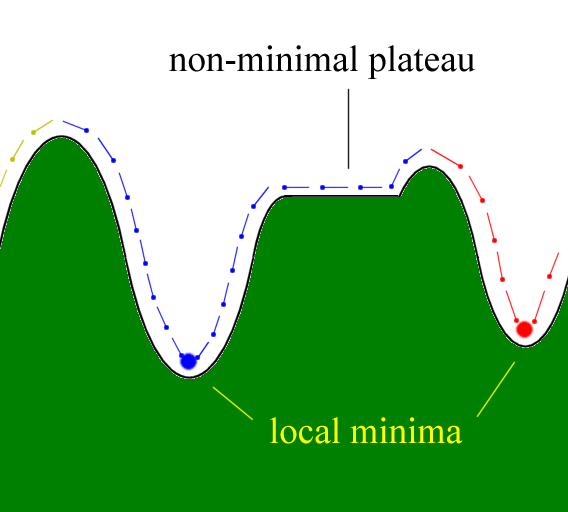
\includegraphics[height=5cm]{segmentation/segmentation-watershed-rainfallingconcept-a.png}}%
	%
	\hspace{4mm}%
	%
	\subfigure[The division of the landscape into catchment basins]
	{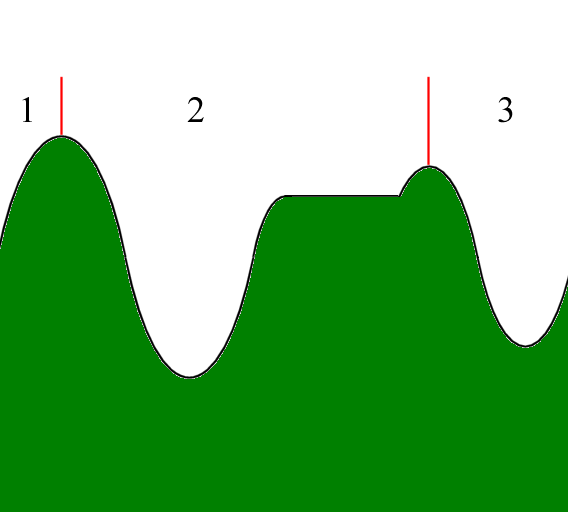
\includegraphics[height=5cm]{segmentation/segmentation-watershed-rainfallingconcept-b.png}}%
\caption{The rainfalling concept of the watershed transform}
\label{fig:segmentation-watershed-rainfallingconcept}
\end{stusubfig}
%---

%---
\begin{stusubfig}{p}
	\subfigure[Beginning the flooding]
	{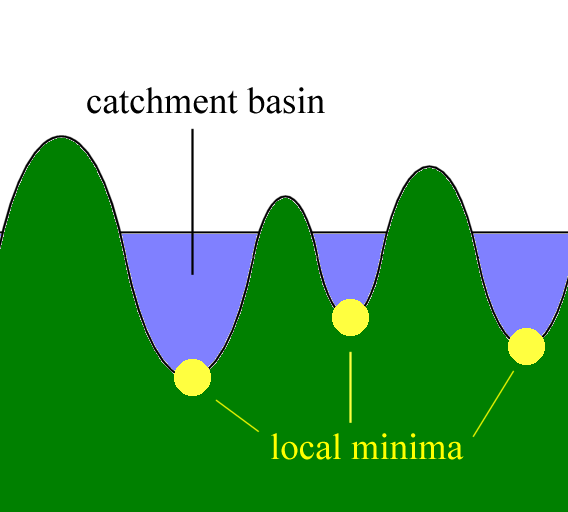
\includegraphics[height=5cm]{segmentation/segmentation-watershed-floodingconcept-a.png}}%
	%
	\hspace{4mm}%
	%
	\subfigure[Two catchment basins meet]
	{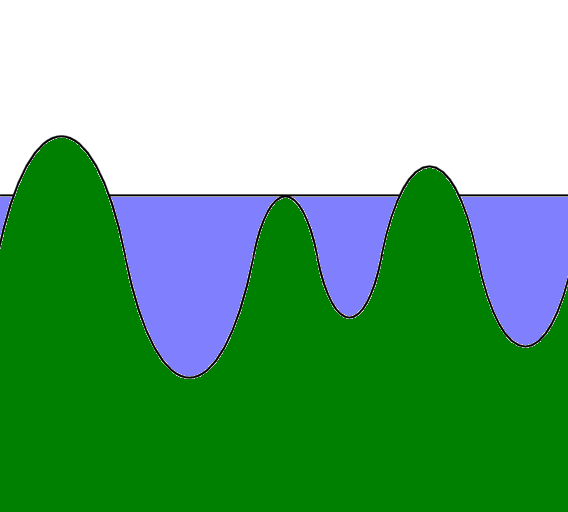
\includegraphics[height=5cm]{segmentation/segmentation-watershed-floodingconcept-b.png}}%
	%
	\hspace{4mm}%
	%
	\subfigure[Building a watershed at the join point]
	{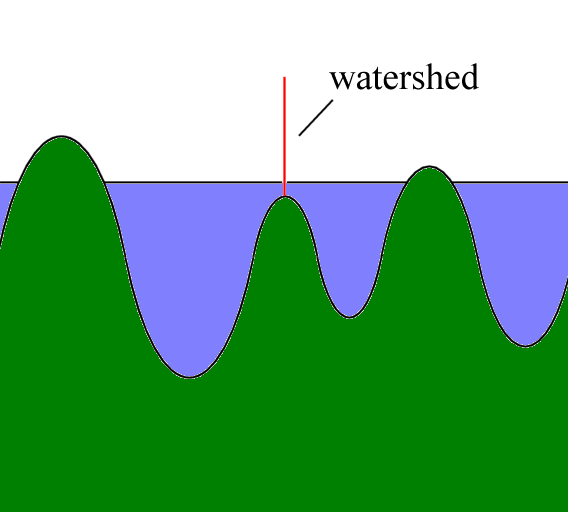
\includegraphics[height=5cm]{segmentation/segmentation-watershed-floodingconcept-c.png}}%
	%
	\hspace{4mm}%
	%
	\subfigure[The division of the landscape into catchment basins]
	{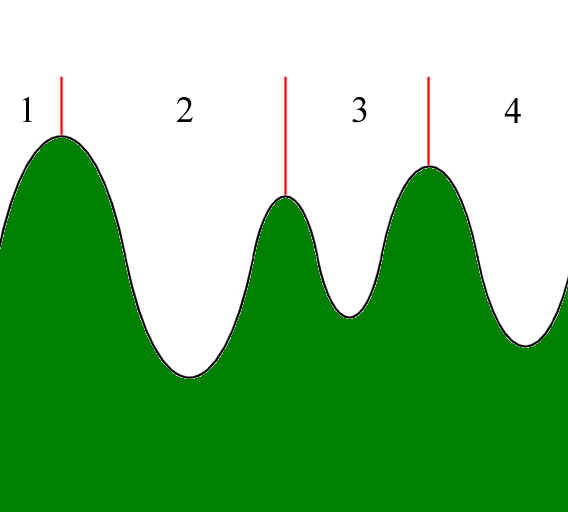
\includegraphics[height=5cm]{segmentation/segmentation-watershed-floodingconcept-d.png}}%
\caption{The flooding concept of the watershed transform}
\label{fig:segmentation-watershed-floodingconcept}
\end{stusubfig}
%---

\index{watershed transform!concept|)}

%################################################
\subsection{Segmenting Grey-Scale Images}
\label{subsec:segmentation-watershed-greyscale}
%################################################

\index{watershed transform!on grey-scale images|(}

The watershed transform is commonly thought of not in the abstract terms just described, but as an image segmentation method. In particular, it is often used to segment grey-scale images. This requires a conceptual mapping that lets us view grey-scale images as landscapes. For example, we can view a 2D, grey-scale image $I$ as a height map (see Figure~\ref{fig:segmentation-watershed-landscapeanalogy}), where the grey value of the image at coordinates $(x,y)$ gives us the height of the landscape at that point. An analogous mapping can be made in higher dimensions (and specifically in three dimensions), although this is harder to visualize. The regions produced by applying an image-based algorithm for a watershed transform to an image correspond to the catchment basins of the discrete landscape to which the image corresponds (see Figure~\ref{fig:segmentation-watershed-regionbasincorrespondence}).

%---
\stufigex{height=6cm}{segmentation/segmentation-watershed-landscapeanalogy.png}{The landscape analogy -- viewing a 2D image as a height map}{fig:segmentation-watershed-landscapeanalogy}{p}
%---

%--
\begin{stusubfig}{p}
	\subfigure[An image]
	{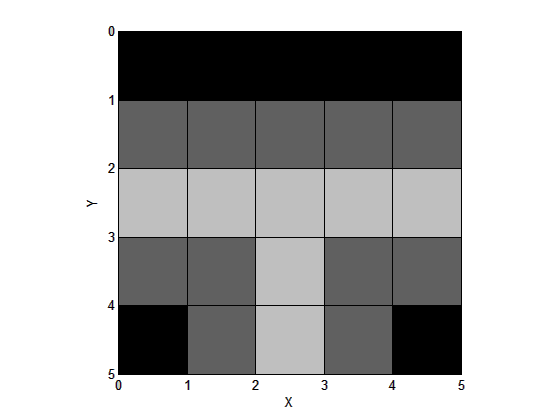
\includegraphics[height=5cm]{segmentation/segmentation-watershed-regionbasincorrespondence-a.png}}%
	%
	\hspace{4mm}%
	%
	\subfigure[The corresponding discrete landscape]
	{\hspace{4mm}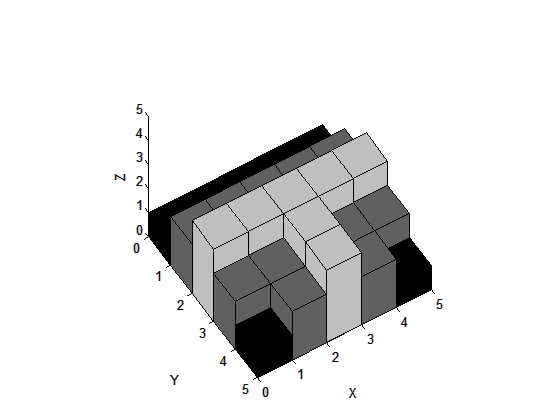
\includegraphics[height=5cm]{segmentation/segmentation-watershed-regionbasincorrespondence-b.png}\hspace{4mm}}%
	%
	\\
	%
	\subfigure[The image after watershed segmentation]
	{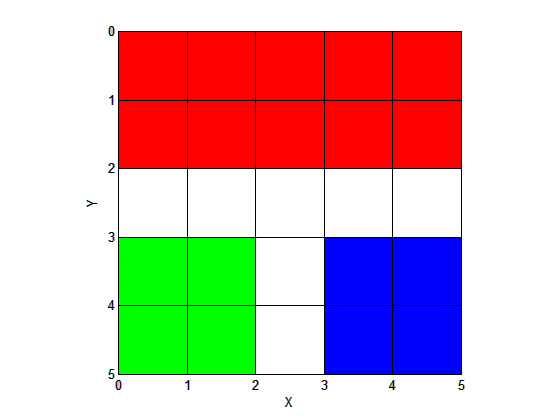
\includegraphics[height=5cm]{segmentation/segmentation-watershed-regionbasincorrespondence-c.png}}%
	%
	\hspace{4mm}%
	%
	\subfigure[The landscape after watershed segmentation]
	{\hspace{4mm}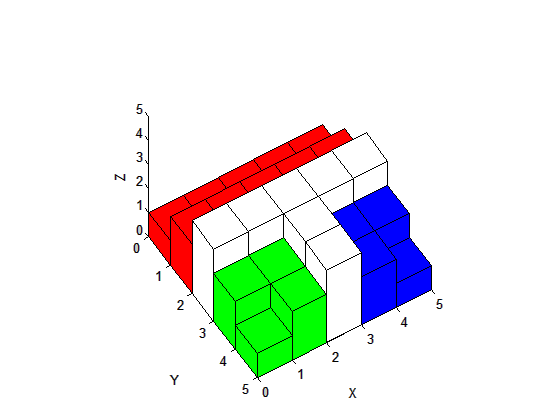
\includegraphics[height=5cm]{segmentation/segmentation-watershed-regionbasincorrespondence-d.png}\hspace{4mm}}%
\caption{Applying a watershed algorithm to an image partitions the image into regions that correspond to the catchment basins of the discrete landscape to which the image corresponds.}
\label{fig:segmentation-watershed-regionbasincorrespondence}
\end{stusubfig}
%--

A variety of different image watershed algorithms are possible (e.g.~\cite{bieniek00,meijster98,osma-ruiz06,rambabu07,stoev00}), but I will focus on Meijster and Roerdink's rainfalling method described in \cite{meijster98}, not least because the ideas behind it translate across to my rainfalling algorithm for the waterfall transform described in \S\ref{subsubsec:segmentation-waterfall-myalgorithm}.

%~~~~~~~~~~~~~~~~~~~~~~~~~~~~~~~~~~~~~~~~~~~~~~~~
\subsubsection{Meijster and Roerdink's Rainfalling Watershed Algorithm}
\label{subsubsec:segmentation-watershed-meijster}
%~~~~~~~~~~~~~~~~~~~~~~~~~~~~~~~~~~~~~~~~~~~~~~~~

\index{watershed transform!Meijster/Roerdink algorithm|(}

%~~~~~~~~~~~~~~~~~~~~~~~
\paragraph{Definitions}
%~~~~~~~~~~~~~~~~~~~~~~~

For the purposes of this algorithm, we define an image to be a function $I: \Omega_{\subset \mathbb{Z}^n} \to \mathbb{Z}$ that maps elements of the domain $\Omega$ to integer grey values. (For instance, a $2$-dimensional $512 \times 512$ image could be defined to have domain $\Omega = \{(x,y) : 0 \le x,y < 512\}$.) A pixel $\mathbf{p} \in \Omega$ is defined to have height $I(\mathbf{p})$ and neighbour set $N(\mathbf{p})$, according to some implementation-defined notion of neighbourhood: usually neighbourhood is defined so that pixels are either 4- or 8-connected in 2D, and 6- or 26-connected in 3D (see Figure~\ref{fig:segmentation-watershed-connectivity}). A singular minimum of an image is a point whose neighbours are all strictly higher than it. Formally, $\mathbf{p}$ is a singular minimum iff $\forall \mathbf{p'} \in N(\mathbf{p}) \cdot I(\mathbf{p'}) > I(\mathbf{p})$. A plateau of an image is a maximal set of two or more connected pixels of equal altitude. A minimal plateau is a plateau from which it is impossible to descend, and a non-minimal plateau is the opposite. Together, the singular minima and minimal plateaux of an image form the local minima of the image.

%---
\begin{stusubfig}{p}
	\subfigure[4-connected (2D)]
	{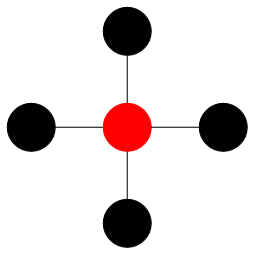
\includegraphics[height=4cm]{segmentation/segmentation-watershed-connectivity-4.png}}%
	%
	\hspace{4mm}%
	%
	\subfigure[8-connected (2D)]
	{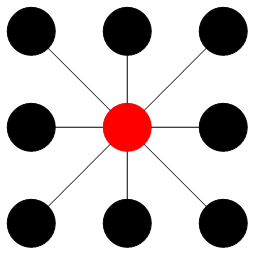
\includegraphics[height=4cm]{segmentation/segmentation-watershed-connectivity-8.png}}%
	%
	\\
	%
	\subfigure[6-connected (3D)]
	{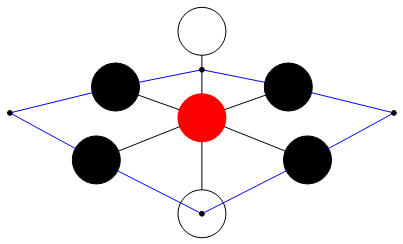
\includegraphics[height=6cm]{segmentation/segmentation-watershed-connectivity-6.png}}%
	%
	\hspace{4mm}%
	%
	\subfigure[26-connected (3D)]
	{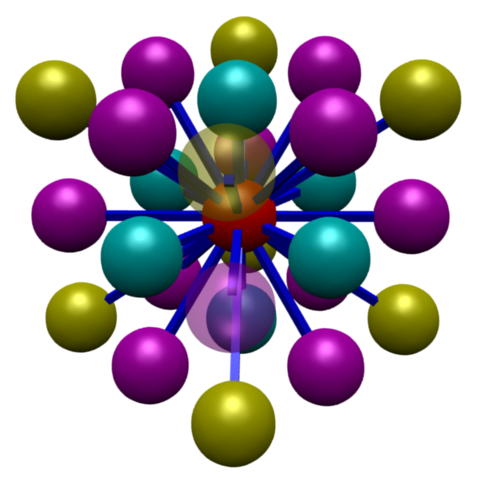
\includegraphics[height=6cm]{segmentation/segmentation-watershed-connectivity-26.png}}%
\caption{Notions of neighbourhood for image pixels in 2D and 3D}
\label{fig:segmentation-watershed-connectivity}
\end{stusubfig}
%---

%---
\stufigex{height=6cm}{segmentation/segmentation-watershed-steepestdescent.png}{The flow direction at a point is ambiguous if it has more than one path of steepest descent}{fig:segmentation-watershed-steepestdescent}{p}
%---

%~~~~~~~~~~~~~~~~~~~~~~~
\paragraph{Overview}
%~~~~~~~~~~~~~~~~~~~~~~~

The approach taken by rainfalling algorithms for the watershed transform, as noted above, is to find a path of steepest descent from each point in the landscape to a local minimum in the landscape (the base of a catchment basin). This is complicated by the fact that there may be non-minimal plateaux (flat areas) in the image: if water were dropped on a pixel in the middle of a non-minimal plateau, the direction in which it would run off would be unclear. To circumvent this problem, the Meijster/Roerdink algorithm starts by transforming the image to make sure every non-minimal pixel has a lower neighbour, thus forming what is known as a lower-complete image. The rest of the algorithm is then split into two stages: in the first stage, each pixel is assigned an arrow pointing to one of its lowest neighbours, and in the second stage, these arrows are followed to find the local minimum associated with each pixel. Each local minimum has a catchment basin, which is defined as all the pixels whose paths of steepest descent lead to it. It is worth observing that points can have more than one path of steepest descent (see Figure~\ref{fig:segmentation-watershed-steepestdescent}): the decision of which one to follow for each point depends on how the arrows are assigned. Different choices lead to subtly different results, and it is important that arrows are at the very least assigned deterministically, so that the results don't vary from one run of the algorithm to the next.

%~~~~~~~~~~~~~~~~~~~~~~~
\paragraph{The Lower-Complete Transformation}
%~~~~~~~~~~~~~~~~~~~~~~~

The lower-complete transformation described by Meijster and Roerdink in \cite{meijster98} essentially works by raising all plateau pixels by their distance from the edge of their plateau (see Figure~\ref{fig:segmentation-watershed-plateau}(a)). Doing this na\"ively doesn't work in the general case, because it can change the ordering of the plateau pixels with respect to the other pixels in the image (see Figure~\ref{fig:segmentation-watershed-plateau}(b)). The solution is to find the maximum amount by which a plateau pixel should be raised, and multiply all pixels by that before raising any plateau pixels: this has the effect of spreading the landscape heights out to accommodate the new altitudes in the middle (see Figure~\ref{fig:segmentation-watershed-plateau}(c)).

The lower-complete transformation can be implemented straightforwardly using a breadth-first search (see Listing~\ref{code:segmentation-watershed-lowercomplete}). The results of the transformation are illustrated in Figure~\ref{fig:segmentation-watershed-example}: an example image is shown in (a), and the result of making it lower-complete is shown in (b).\fxnote{[IDV] Expand/explain [this paragraph].}

%---
\begin{stusubfig}{p}
\subfigure[The `intuition' is to raise plateau pixels by their distance from the edge]
	{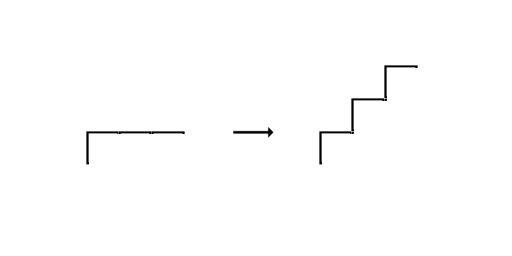
\includegraphics[width=.45\linewidth]{segmentation/segmentation-watershed-plateau-a.png}}%
	%
	\hspace{4mm}%
	%
	\subfigure[Doing this na\"ively can change the height ordering of the pixels in the image]
	{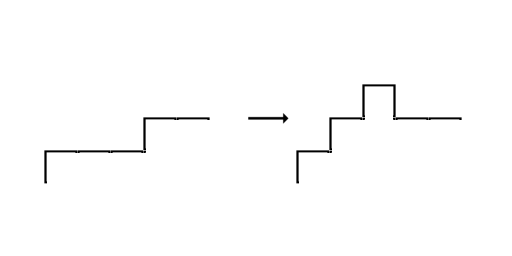
\includegraphics[width=.45\linewidth]{segmentation/segmentation-watershed-plateau-b.png}}%
	%
	\hspace{4mm}%
	%
	\subfigure[This can be fixed by spreading the landscape out prior to raising the pixels]
	{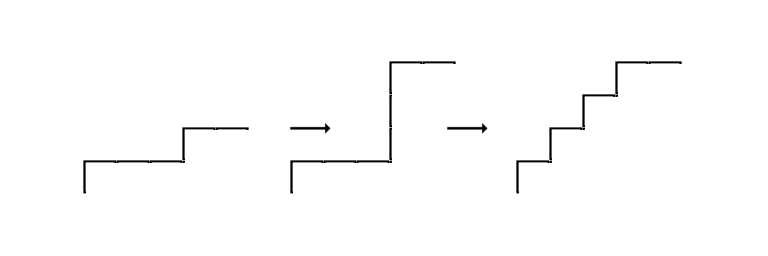
\includegraphics[width=.45\linewidth]{segmentation/segmentation-watershed-plateau-c.png}}%
\caption{A solution to the non-minimal plateau problem}
\label{fig:segmentation-watershed-plateau}
\end{stusubfig}
%---

%---
\begin{stusubfig}{p}
	\subfigure[The original image]{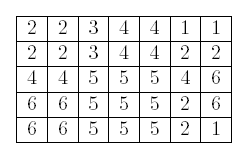
\includegraphics[height=4cm]{segmentation/segmentation-watershed-example-a.png}}%
	%
	\hspace{4mm}%
	%
	\subfigure[The lower-complete image]{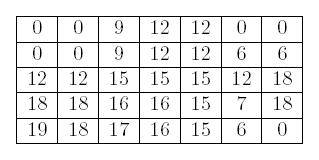
\includegraphics[height=4cm]{segmentation/segmentation-watershed-example-b.png}}%
	%
	\hspace{4mm}%
	%
	\subfigure[The arrows on each pixel]{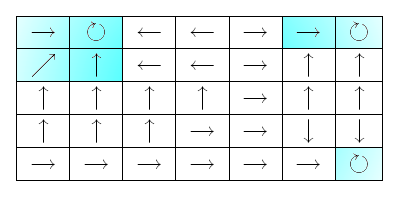
\includegraphics[height=4cm]{segmentation/segmentation-watershed-example-c.png}}%
	%
	\hspace{4mm}%
	%
	\subfigure[The final labelling]{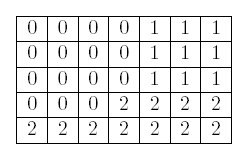
\includegraphics[height=4cm]{segmentation/segmentation-watershed-example-d.png}}%
\caption{An example illustrating the stages of the Meijster/Roerdink watershed algorithm}
\label{fig:segmentation-watershed-example}
\end{stusubfig}
%---

%---
\begin{stulisting}[p]
\caption{The Lower-Complete Transformation}
\label{code:segmentation-watershed-lowercomplete}
\begin{lstlisting}[style=Default]
function build_lower_complete
: (image : Image<$\Omega$,int>) $\to$ Image<$\Omega$,int>

	var lc : Image<$\Omega$,int>;
	var queue : Queue<PixelCoords>;

	// Initialise the queue with pixels that have a lower neighbour.
	for each p : PixelCoords $\in$ N(p)
		lc(p) := 0;
		for each neighbour : PixelCoords $\in$ N(p)
			if image(neighbour) < image(p) then
				queue.push(p);
				// To prevent it being queued twice.
				lc(p) := -1;
				break;

	// Compute a function which indirectly indicates the amount by which
	// we need to raise the plateau pixels (see the paper by Meijster and
	// Roerdink for more details).
	var p : PixelCoords;
	var dist : int(1);
	var marker : PixelCoords(-1,-1);
	queue.push(marker);
	while not queue.empty()
		p := queue.pop();
		if p = marker then
			if not queue.empty() then
				queue.push(marker);
				dist := dist + 1;
		else
			lc(p) := dist;
			for each neighbour : PixelCoords $\in$ N(p)
				// If the neighbouring pixel is at the
				// same altitude and has not yet been
				// processed.
				if image(neighbour) = image(p) and lc(neighbour) = 0 then
					queue.push(neighbour);
					// To prevent it being queued twice.
					lc(neighbour) := -1;
	
	// Compute the final lower-complete function. Note that at this point,
	// dist holds the amount by which we want to multiply the base image.
	for each p : PixelCoords $\in$ $\Omega$
		if lc(p) $\ne$ 0 then
			lc(p) := dist * image(p) + lc(p) - 1;

	return lc;
\end{lstlisting}
\end{stulisting}
%---

%~~~~~~~~~~~~~~~~~~~~~~~
\paragraph{Arrow Assignment}
%~~~~~~~~~~~~~~~~~~~~~~~

The remainder of the algorithm is designed to calculate paths of steepest descent for each point in the image. Evidently the na\"ive approach of finding a steepest path for each point in turn would be computationally costly, but this is unnecessary as the problem of finding steepest paths exhibits optimal substructure. Because of this, it suffices to assign an arrow to each pixel to indicate the direction of a steepest path through that pixel and then follow the arrows to find steepest paths for each pixel.

The arrow assignment process works as follows. Firstly, one of the pixels in each minimal plateau is chosen as a canonical element of that plateau. For each pixel, an arrow is then assigned according to its type:
%
\begin{enumerate}
\item If the pixel is a singular minimum, or the canonical element\fxnote{[IDV] CRITERIA?} of a minimal plateau, then its arrow is a self-loop.
\item If the pixel is a non-canonical element of a minimal plateau, then its arrow points directly to the canonical element of the plateau.
\item The arrow of any other pixel points to a lowest neighbour of that pixel.
\end{enumerate}
%
The implementation (see Listing~\ref{code:segmentation-watershed-arrowassignment}) uses Tarjan's disjoint set forest data structure (see Appendix~\ref{chap:appendixds}). The idea is to combine all the minimum points into their respective local minima using this data structure, and make all the other non-minimal points point to one of their lower neighbours. We also take the opportunity to numerically label all the canonical points of minimal plateaux during this phase of the process. The results of the arrow assignment are shown in Figure~\ref{fig:segmentation-watershed-example}(c).

%---
\begin{stulisting}[p]
\caption{Arrow Assignment}
\label{code:segmentation-watershed-arrowassignment}
\begin{lstlisting}[style=Default]
function construct_arrows
: (lc : Image<$\Omega$,int>) $\to$ (Image<$\Omega$,PixelCoords>, Image<$\Omega$,int>)

	var arrows : Image<$\Omega$,PixelCoords>;
	var labels : Image<$\Omega$,int>;

	// Add all the minimum points to a disjoint set forest.
	var labelCount : int(0);
	var minima : DisjointSetForest<PixelCoords>;
	for each p : PixelCoords $\in \Omega$
		if lc(p) = 0 then
			labels(p) := labelCount;
			labelCount := labelCount + 1;
			minima.add_element(p);

	for each p : PixelCoords $\in \Omega$
		if lc(p) = 0 then
			// Union any neighbouring minimum points into the same local minimum.
			for each neighbour : PixelCoords $\in$ N(p)
				if lc(neighbour) = 0 then
					minima.union_sets(labels(p), labels(neighbour));
		else
			// Find a lowest neighbour and make this point's arrow point to it.
			var lowestNeighbour : PixelCoords(-1,-1);
			var lowestNeighbourValue : int($\infty$)
			for each neighbour : PixelCoords $\in$ N(p)
				if lc(neighbour) < lowestNeighbourValue then
					lowestNeighbour := neighbour;
					lowestNeighbourValue := lc(neighbour);
			// There will always be a lowest neighbour here since the function's
			// lower-complete.
			arrows(p) := lowestNeighbour;

	// Assign new labels to the canonical points of the regional minima and make
	// the arrows of the non-canonical points point to them.
	labelCount := 1;
	for each p : PixelCoords $\in \Omega$
		if lc(p) $\ne$ 0 then continue
		var root : int := minima.find_set(labels(p));
		if root = labels(p) then
			// This is a canonical point.
			arrows(p) := p;
			labels(p) := labelCount;
			labelCount := labelCount + 1;
		else
			arrows(p) := minima.value_of(root);

	return (arrows, labels);
\end{lstlisting}
\end{stulisting}
%---

%---
\begin{stulisting}[p]
\caption{Labelling}
\label{code:segmentation-watershed-labelling}
\begin{lstlisting}[style=Default]
function resolve_all
: (arrows : Image<$\Omega$,PixelCoords>; labels : ref Image<$\Omega$,int>) $\to \emptyset$

	for each p : PixelCoords $\in \Omega$
		resolve_pixel(p, arrows, labels)

function resolve_pixel
: (p : PixelCoords;
	 arrows : Image<$\Omega$,PixelCoords>;
	 labels : ref Image<$\Omega$,int) $\to$ PixelCoords

	var parent : PixelCoords := arrows(p);
	if parent $\ne$ p then
		parent := resolve_pixel(parent, arrows, labels);
		labels(p) := labels(parent);
	return parent;
\end{lstlisting}
\end{stulisting}
%---

%~~~~~~~~~~~~~~~~~~~~~~~
\paragraph{Labelling}
%~~~~~~~~~~~~~~~~~~~~~~~

Once arrows have been assigned to all the pixels in the image, the paths they form from each pixel to a local minimum are followed and each pixel is assigned the label of the appropriate local minimum (see Listing~\ref{code:segmentation-watershed-labelling}). The process can be made more efficient by using path compression when following a path to a minimum (i.e.~we make all the arrows on the path point to the minimum once we've found it). This bears some similarities to the way disjoint set forests are implemented (see Appendix~\ref{chap:appendixds}). The output of Meijster/Roerdink algorithm is a labelled image, as shown in Figure~\ref{fig:segmentation-watershed-example}(d). It is thus an algorithm which outputs catchment basins rather than watershed lines.

\index{watershed transform!Meijster/Roerdink algorithm|)}
\index{watershed transform!on grey-scale images|)}

%################################################
\subsection{Segmenting CT Images}
\label{subsec:segmentation-watershed-ct}
%################################################

\index{watershed transform!on CT images|(}

Having seen how to apply a watershed transform to generic grey-scale images, we can now turn our sights to the specific images that are the real target of this thesis -- computerised tomography (CT) scans of the abdomen. As described in the introduction, CT images are merely grey-scale images whose pixels are scalar values on a particular scale, namely the Hounsfield scale\index{Hounsfield!scale}, and as such, they can in principle be segmented using the type of grey-scale image watershed algorithm just described. However, a number of issues must first be tackled in order to obtain desirable results.\fxnote{[IDV] This is a bit abrupt. You need a transition paragraph explaining why you move `away' from M+R's algorithm.}

%~~~~~~~~~~~~~~~~~~~~~~~~~~~~~~~~~~~~~~~~~~~~~~~~
\subsubsection{Smoothness}
\label{subsubsec:segmentation-watershed-ct-smoothness}
%~~~~~~~~~~~~~~~~~~~~~~~~~~~~~~~~~~~~~~~~~~~~~~~~

A key issue which arises when applying the watershed to CT images is their lack of smoothness (especially in the presence of noise). The images have many local minima, most of them spurious: this is analogous to working with a highly pock-marked landscape (see Figure~\ref{fig:segmentation-watershed-pockmarkedlandscape}). Such a landscape will have many catchment basins; running a watershed algorithm on a non-smooth image will thus greatly over-segment it (each minor dimple in the landscape gets treated as a separate catchment basin). Figure~\ref{fig:segmentation-watershed-adfexample}(e), which shows the result of running my implementation of Meijster and Roerdink's watershed algorithm on a raw CT image, illustrates this problem -- note the vast number of individual regions with little semantic meaning.

%---
\stufigex{width=16cm}{segmentation/segmentation-watershed-pockmarkedlandscape.jpg}{Non-smooth images are analogous to a pock-marked landscape: they have large numbers of catchment basins, most of which are just small hollows that are of limited relevance. The image is courtesy of JAXA (see http://wms.selene.jaxa.jp/selene_viewer/terms_of_use_e.html) and was taken by the Kaguya lunar probe.}{fig:segmentation-watershed-pockmarkedlandscape}{p}
%---

The solution lies partly in smoothing the original image (a pre-processing step), and partly in merging the large number of small regions generated by the watershed algorithm together into larger regions with more semantic meaning (a post-processing step for which we use the waterfall transform, described later). The goal in smoothing the watershed input is to remove spurious local minima whilst preserving important semantic information in the image. In particular, it is important to try and preserve boundaries between adjacent features, which may not be as pronounced as we would prefer even at the best of times. To do this, edge-preserving filtering techniques such as \emph{anisotropic diffusion filtering} \cite{perona90} or \emph{bilateral filtering} \cite{tomasi98} may be used. For my purposes, I compared the implementations of anisotropic diffusion filtering and bilateral filtering found in the Insight Toolkit \cite{itk}, and selected anisotropic diffusion filtering for use based on its superior results and speed on my images.

%~~~~~~~~~~~~~~~~~~~~~~~
\paragraph{Anisotropic Diffusion Filtering}
%~~~~~~~~~~~~~~~~~~~~~~~

\index{anisotropic diffusion filtering|(}

The anisotropic diffusion filtering (ADF) technique was originally introduced by Perona and Malik in \cite{perona90}. The basic idea stems from the fact that solving a heat equation of the form
%
\[
\pd{I(x,y,t)}{t} = \nabla^2 I(x,y,t) \equiv \nabla \cdot \nabla I(x,y,t)
\]
%
on an image $I_0(x,y)$, by setting $I(x,y,0) = I_0(x,y)$ as the initial condition, is equivalent to convolving $I_0$ with a Gaussian of standard deviation $\sqrt{2t}$. (In other words, by finding the solution to the heat equation at a time $t_0$, we are effectively blurring the image with the corresponding Gaussian.) Perona and Malik's idea was that by replacing $\nabla I(x,y,t)$ in the equation with $C \nabla I(x,y,t)$, for some $C$\fxnote{[IDV] Constant? Function?}, the results of solving the heat equation could be influenced to depend on where we expect the edges in the original image to be. In particular, if we assume that the gradient magnitude of the original image provides a reasonable estimate of where the edges are, then we can write $C = c(|\nabla I(x,y,t)|)$, for some function $c$, giving us the anisotropic diffusion equation
%
\[
\pd{I(x,y,t)}{t} = \nabla \cdot c(|\nabla I(x,y,t)|) \nabla I(x,y,t).
\]
%
We thereby introduce a prior expectation of where we expect the edges to be into the equation, allowing us to influence the smoothing process so as to preserve them. The key to this is in how we specify $c$. We want the image to be blurred less where $|\nabla I|$ is large (i.e.~where we presume there to be edges), so $c$ must yield a small value for large $|\nabla I|$ and a larger value for small $|\nabla I|$. There are an infinite number of functions which would satisfy this, but an effective $c$ from the literature (and, in particular, the one used in the Insight Toolkit \cite{itk} implementation I used) is given by
%
\[
c(|\nabla I|) = e^{-\frac{|\nabla I|^2}{2k^2}},
\]
%
where $k$ is simply a parameter used to control the extent to which smoothing is affected by the gradient magnitude image. Overall, ADF as implemented in ITK thus takes two parameters: a time $t_0$, which indirectly specifies the standard deviation of the Gaussian used, and $k$, as just mentioned.

The results of smoothing using ADF are shown in Figure~\ref{fig:segmentation-watershed-adfexample}, which compares the gradient magnitude and watershed results of an unsmoothed image with that of an image smoothed using ADF, in order to show the effects on the edges and resulting segmentation. The important thing to note is that ADF has smoothed away all the unnecessary detail in the middle of the organs, whilst preserving what boundaries there were around them. This makes the resulting segmentation far better than it would have been without smoothing.

%---
\begin{stusubfig}{p}
	\subfigure[Unsmoothed image]
	{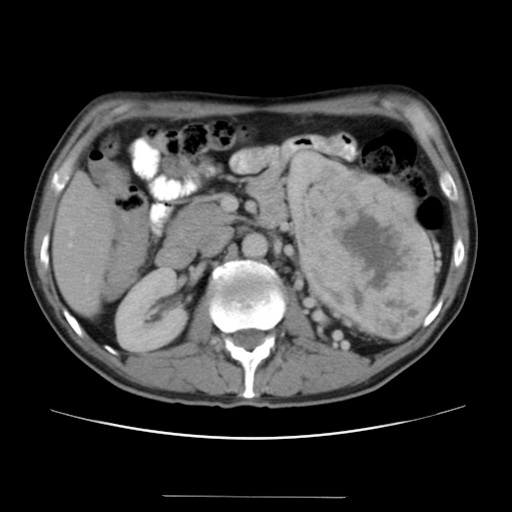
\includegraphics[height=6cm]{segmentation/segmentation-watershed-adfexample-unsmoothed.png}}%
	%
	\hspace{4mm}%
	%
	\subfigure[Smoothed image]
	{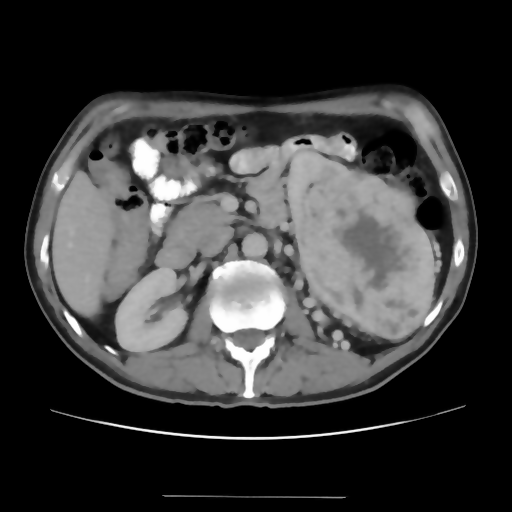
\includegraphics[height=6cm]{segmentation/segmentation-watershed-adfexample-smoothed.png}}%
	%
	\\
	%
	\subfigure[Gradient magnitude of the unsmoothed image]
	{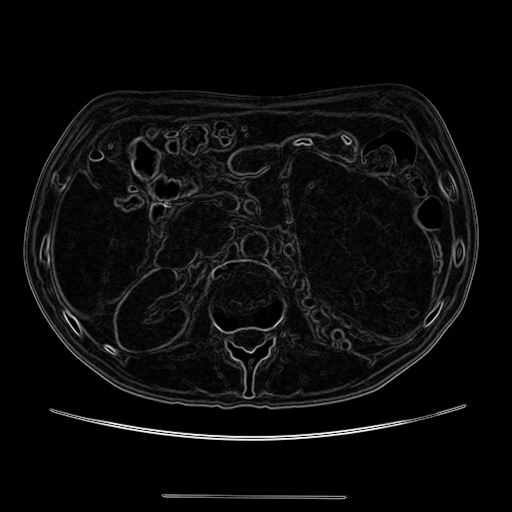
\includegraphics[height=6cm]{segmentation/segmentation-watershed-adfexample-unsmoothedgm.png}}%
	%
	\hspace{4mm}%
	%
	\subfigure[Gradient magnitude of the smoothed image]
	{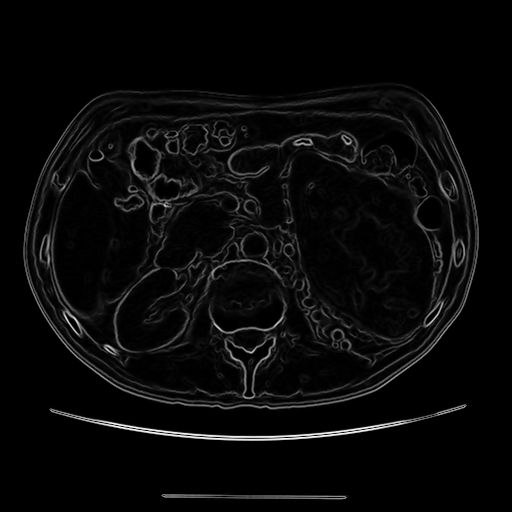
\includegraphics[height=6cm]{segmentation/segmentation-watershed-adfexample-smoothedgm.png}}%
	%
	\\
	%
	\subfigure[Watershed of the unsmoothed image]
	{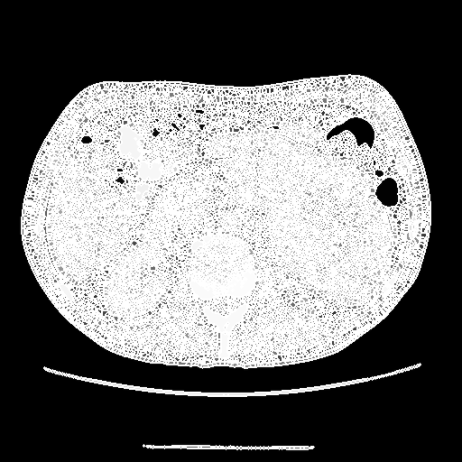
\includegraphics[height=6cm]{segmentation/segmentation-watershed-adfexample-unsmoothedws.png}}%
	%
	\hspace{4mm}%
	%
	\subfigure[Watershed of the smoothed image]
	{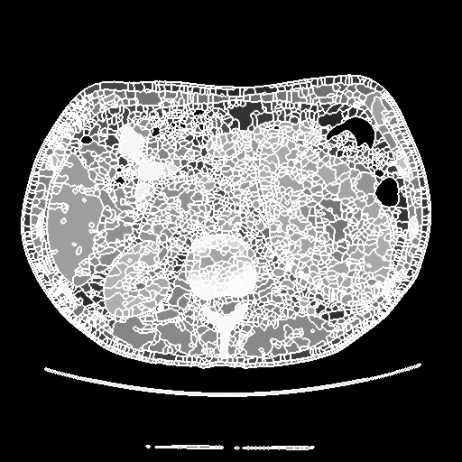
\includegraphics[height=6cm]{segmentation/segmentation-watershed-adfexample-smoothedws.png}}%
\caption{The results of running a watershed algorithm on an image smoothed by anisotropic diffusion filtering (ADF) are far superior, because ADF smoothes away all the unnecessary detail within features whilst preserving the crucial edges between them.}
\label{fig:segmentation-watershed-adfexample}
\end{stusubfig}
%---

\index{anisotropic diffusion filtering|)}

%~~~~~~~~~~~~~~~~~~~~~~~~~~~~~~~~~~~~~~~~~~~~~~~~
\subsubsection{Features vs. Catchment Basins}
%~~~~~~~~~~~~~~~~~~~~~~~~~~~~~~~~~~~~~~~~~~~~~~~~

A further issue when dealing with CT images is that whilst grey-scale image watershed algorithms like the one described earlier segment the image into regions which correspond to the catchment basins of the discrete landscape associated with the image, it is unusual for these catchment basins to correspond directly to features of interest in our input image. For instance, if we're trying to segment a kidney in a CT image, there is no reason to suppose that the kidney will correspond to a catchment basin in the landscape: applying a watershed algorithm directly, therefore, will not in general yield useful results.

What we need is a way of transforming our input image into one where the features of interest correspond more directly to its catchment basins. Unfortunately there is no domain-independent solution to this (it depends on the type of image we are segmenting and the sort of features in which we're interested), but it is possible to come up with suitable transformations on a domain-by-domain basis. Our goal in the case of CT images is generally to segment things like organs. The grey value in the images tends to vary relatively slowly across individual organs and relatively quickly at their edges because of the tissue types involved (another way of saying this is that the organs tend to be homogeneous). The intuition is therefore that the value of the gradient magnitude is relatively low within organs, and relatively high at their edges (e.g.~see Figures~\ref{fig:segmentation-watershed-adfexample}(c) and (d)), so a much better correspondence between organs and catchment basins (i.e.~a much more useful segmentation result) can be obtained by running the watershed on the gradient magnitude image instead of the original input. It should be noted, however, that this scheme is of less use when the goal is to segment inhomogeneous features like tumours.

%---
\stufigex{width=.95\linewidth}{segmentation/segmentation-watershed-windowing.png}{The chosen CT window (centre 40, width 400) is mapped to the available grey values}{fig:segmentation-watershed-windowing}{p}
%---

%---
\begin{stusubfig}{p}
	\subfigure[Segmentation of a Hounsfield image before windowing]
	{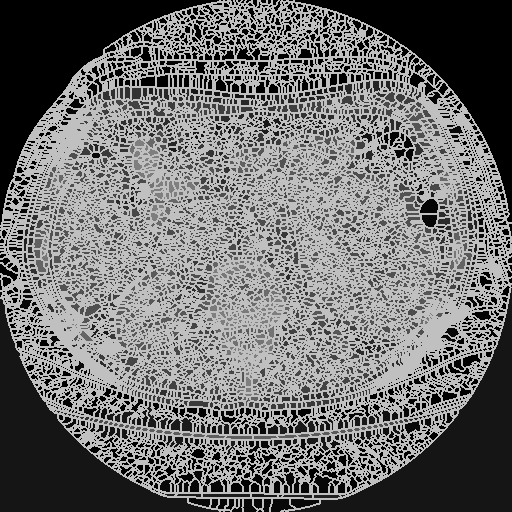
\includegraphics[width=.45\linewidth]{segmentation/segmentation-watershed-hounsfieldvswindowed-h.png}}%
	%
	\hspace{4mm}%
	%
	\subfigure[Segmentation of the same image after windowing]
	{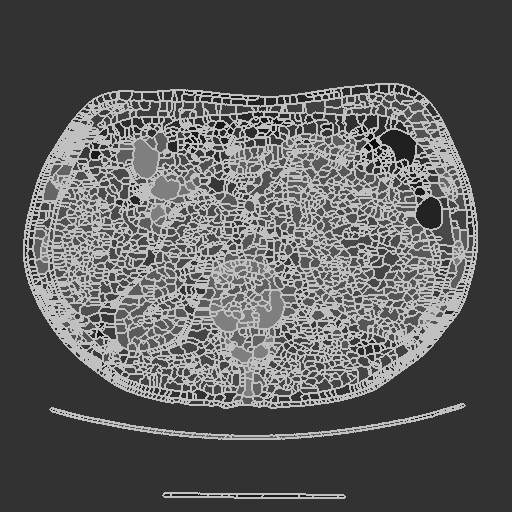
\includegraphics[width=.45\linewidth]{segmentation/segmentation-watershed-hounsfieldvswindowed-w.png}}%
\caption{Windowing images before segmenting them leads to a less pronounced oversegmentation -- note in particular the generally larger regions in (b)}
\label{fig:segmentation-watershed-hounsfieldvswindowed}
\end{stusubfig}
%---

%~~~~~~~~~~~~~~~~~~~~~~~~~~~~~~~~~~~~~~~~~~~~~~~~
\subsubsection{Hounsfield Units and Windowing}
\label{subsubsec:segmentation-watershed-ct-windowing}
%~~~~~~~~~~~~~~~~~~~~~~~~~~~~~~~~~~~~~~~~~~~~~~~~

\index{windowing|(}

\index{Hounsfield!scale|(textbf}

A final issue to contend with when working with CT images concerns the Hounsfield scale used for their pixel values. These values, measured in Hounsfield Units (HU), are based on the radiodensity of materials with respect to water, and range from $-1024$ to $3071$. Materials that have a lower radiodensity than water, such as fatty tissue, have negative Hounsfield values; conversely, those with a greater radiodensity than water, such as muscle, have positive values. On this scale, for example, air is at $-1000$ HU, whereas bone appears at $400$ HU or more. The scale is calibrated so that water itself is at $0$ HU.

\index{Hounsfield!scale|)textbf}

Having the scanners calibrated to produce images whose pixel values are on a fixed scale with real-world meaning is extremely helpful, but in order to diagnose patients, radiologists need to be able to distinguish between different types of tissue on a viewable image. Unfortunately, there is a limit to how many grey values can be distinguished by the human eye, and the Hounsfield range is too wide ($> 4000$ distinct values) for Hounsfield images to be directly used for diagnostic purposes. (Looking at things another way, viewing a Hounsfield image directly would be equivalent to looking at an image with extremely low contrast.) For this reason, before being viewed by a radiologist, Hounsfield images are subjected to a process known as \emph{windowing}.

Windowing is essentially a method for controlling the brightness and contrast of an image in a way that makes practical sense to radiologists. Rather than viewing the entire Hounsfield scale, the radiologist can select a window (a numerical interval) on the scale which is mapped to the available grey values (see Figure~\ref{fig:segmentation-watershed-windowing}). The position and size of the window are controlled by two parameters, known respectively as the \emph{window level} (L) and \emph{window width} (W). With the window set, the Hounsfield image can then be transformed into a human-viewable grey-scale image. For example, if we were working with 8-bit greyscale images (with $0$ being black and $2^8 - 1 = 255$ being white), then pixels with Hounsfield value $\le L - W/2$ would be mapped to $0$ and those with value $\ge L + W/2$ would be mapped to $255$, with pixel values in between being mapped using the formula:
%
\[
\mbox{Out} = \mbox{Round}\left( (\mbox{In} - L) \times \frac{255}{W} + 127.5 \right)
\]
%
The reason windowing is a sensible way for radiologists to control the brightness and contrast of an image (rather than just adjusting them directly) is that it allows them to focus on an interesting part of the scale. For instance, when diagnosing kidney tumours, it is common to use a window level of $40$ and a window width of $400$ in order to focus on organs made of soft tissue (like the kidneys). A window like $40/400$ would thus be referred to as a soft tissue window. Different windows are used for other types of investigation (e.g.~when looking at lung images), and it is common for appropriate window settings chosen by a radiologist to be stored with each image as meta-data.\fxnote{[IDV] And they therefore get trained to know/recognise these values.}

Windowing makes a practical difference for the purposes of segmentation. In particular, it is possible to work with either the original Hounsfield image or a windowed version of it, and these yield different results. It is noticeable that segmenting a windowed image (using an appropriately chosen window, such as the one stored with the image) tends to work better in practice, in that it produces a less pronounced oversegmentation of the image (see Figure~\ref{fig:segmentation-watershed-hounsfieldvswindowed}). This may seem surprising, since there is effectively less information in the windowed image than the original, but there is a logical explanation. When the width of window chosen is greater than the width of the greyscale range, the process of windowing will map more than one Hounsfield value to the same grey-scale output (one reason why there is a loss of information involved). This has the effect of removing some of the spurious local minima in the image, which improves the resulting watershed segmentation. In short, whilst we are losing some of the information from the original Hounsfield image, the information we are losing was actually hindering the segmentation rather than helping it.

\index{windowing|)}

%~~~~~~~~~~~~~~~~~~~~~~~~~~~~~~~~~~~~~~~~~~~~~~~~
\subsubsection{Summary}
%~~~~~~~~~~~~~~~~~~~~~~~~~~~~~~~~~~~~~~~~~~~~~~~~

To segment a CT image using the watershed transform, then, we first window it using appropriate window settings (generally speaking, the ones stored with the image by a radiologist) in order to obtain a more conventional grey-scale image. We next smooth it using anisotropic diffusion filtering and then pass it through a gradient magnitude filter to try and establish a reasonable correspondence between features of interest in the image and catchment basins in the discrete landscape associated with it. Finally, we run an image watershed algorithm on this smoothed, gradient magnitude image: in our case\fxnote{[IDV] [This sentence reads slightly weirdly]}, we use the Meijster/Roerdink algorithm, which produces an image of numeric labels. As we will see in \S\ref{sec:segmentation-ipfconstruction}, this labelled image is what we need to construct the lowest branch layer of an IPF for the image. The remainder of the IPF will be constructed using the waterfall transform, which will now be introduced.

\index{watershed transform!on CT images|)}
\index{watershed transform|)}

\clearpage

%##################################################################################################
\section{The Waterfall Transform}
\label{sec:segmentation-waterfall}
%##################################################################################################

\index{waterfall transform|(}

%################################################
\subsection{Motivation}
%################################################

\index{waterfall transform!motivation|(}

The watershed transform segments a landscape into its catchment basins, but, as we have seen, this often produces a segmentation that contains far too many regions to be useful for the specific application in which we're interested (segmenting CT images, for example). In the specific context of images, pre-processing the image with an edge-preserving filter helps alleviate the problem somewhat, but fails to completely solve it.

One method that seeks to solve this problem is the so-called `watershed-from-markers' approach \cite{meyer90}, as briefly discussed in Chapter~\ref{chap:background}. The idea behind this is to specify a priori that only certain local minima in the landscape are semantically interesting by placing markers on them. Conceptually, we then fill in all the unmarked minima and keep only the marked ones, before performing a normal watershed on the result (see Figure~\ref{fig:segmentation-waterfall-watershedfrommarkers}), although this is not how the approach tends to be implemented in practice. An example implementation can be found in e.g.~\cite{felkel01}. (Alternatively, consider an approach whereby we flood the landscape from the local minima and only add watersheds when two \emph{marked} catchment basins would otherwise meet.) We can thus constrain the watershed to produce an output with a certain number of regions in it (solving the problem of oversegmentation), provided that we can determine the local minima in which we're interested (the markers) in advance.

%---
\begin{stusubfig}{p}
	\subfigure[Placement of markers (the blue dots)]
	{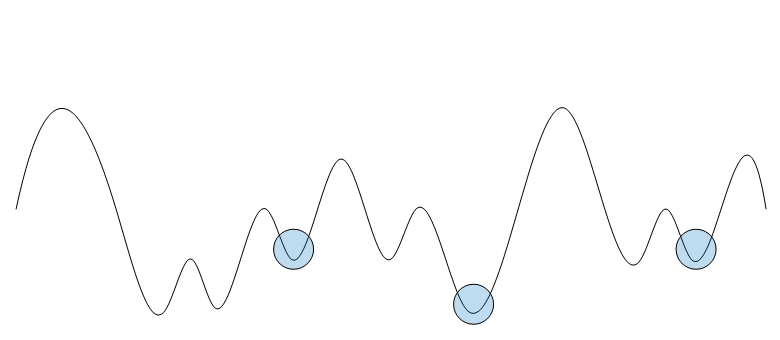
\includegraphics[width=.6\linewidth]{segmentation/segmentation-waterfall-watershedfrommarkers-a.png}}%
	%
	\hspace{4mm}%
	%
	\subfigure[After filling in the unmarked minima]
	{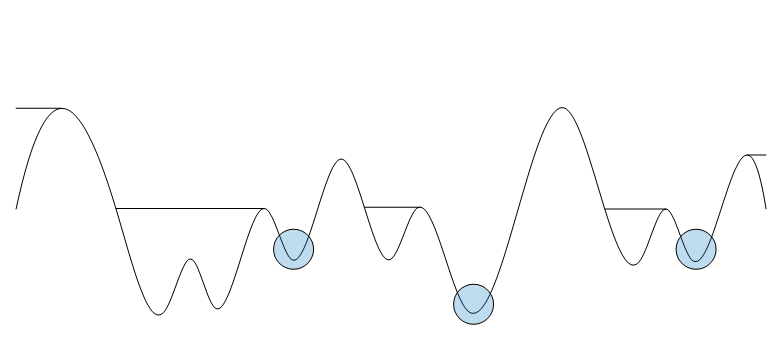
\includegraphics[width=.6\linewidth]{segmentation/segmentation-waterfall-watershedfrommarkers-b.png}}%
	%
	\hspace{4mm}%
	%
	\subfigure[After performing a watershed on the filled landscape]
	{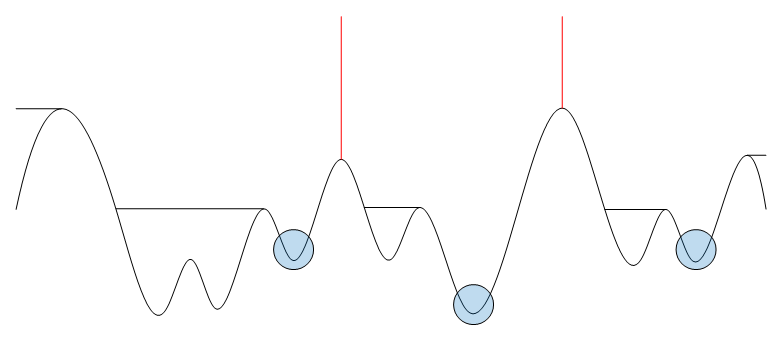
\includegraphics[width=.6\linewidth]{segmentation/segmentation-waterfall-watershedfrommarkers-c.png}}%
\caption{A conceptual view of the watershed-from-markers approach}
\label{fig:segmentation-waterfall-watershedfrommarkers}
\end{stusubfig}
%---

Marker determination can be either manual or automatic, but both approaches have their problems. In the manual approach, the user simply marks the interesting local minima and then runs the segmentation. The downside is that the process is not only time-consuming, but non-intuitive: obtaining a desirable segmentation by placing markers tends to involve a lot of trial-and-error. Automatic approaches are more promising: for example, we could pick the local minima associated with `the n deepest catchment basins' as our markers. The disadvantage in this case is that the results are `all or nothing': a specific automatic marker approach is unlikely to work well for all possible images, and if we get a bad result on a particular image then we have nothing to work with (we are left with a poor segmentation and no obvious way to edit it).

Whilst watershed-from-markers has been used successfully in a variety of situations\fxnote{[IDV] Include examples} (e.g.~\cite{chae07,gonzalez07}), the issues just mentioned make it an undesirable approach to use in the context of the goals outlined in Chapter~\ref{chap:methodology}. A more sensible approach for our purposes is to stick with the output of the normal watershed transform, but post-process it to deal with the oversegmentation. This post-processing comes in the form of a hierarchical watershed-based transform, known as the waterfall.

\index{waterfall transform!motivation|)}

%################################################
\subsection{Concept}
%################################################

\index{waterfall transform!concept|(}

The waterfall transform is a multi-pass, hierarchical segmentation method. It generates a sequence of partitions of a landscape, each coarser (i.e.~containing fewer regions) than the one preceding it. An illustration of this (in image terms) is seen in Figure~\ref{fig:segmentation-waterfall-partitionsequence}, which shows the result of applying four passes of a waterfall algorithm to the watershed result produced from an example image.

%---
\begin{stusubfig}{p}
	\subfigure[The example image]
	{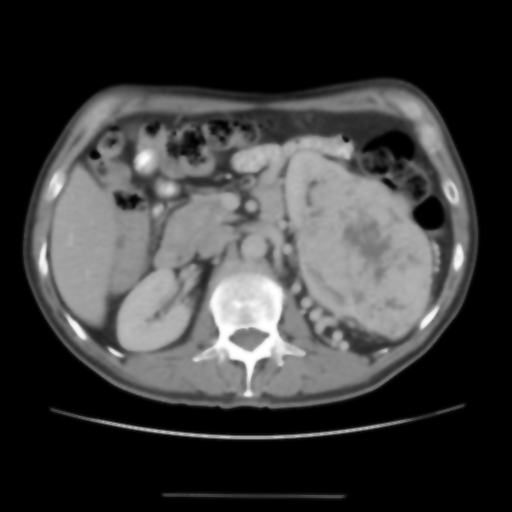
\includegraphics[width=.35\linewidth]{segmentation/segmentation-waterfall-partitionsequence-a.png}}%
	%
	\hspace{4mm}%
	%
	\subfigure[The initial watershed partition]
	{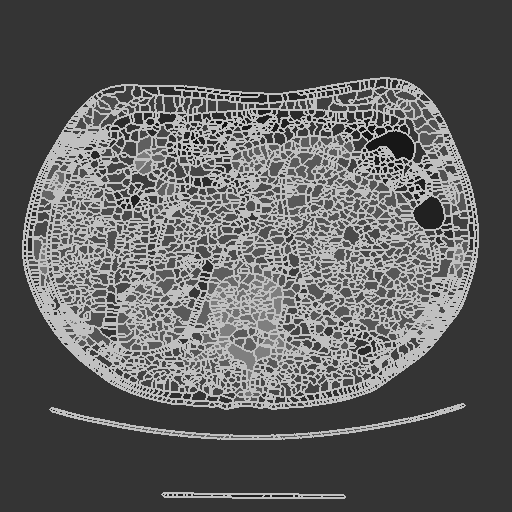
\includegraphics[width=.35\linewidth]{segmentation/segmentation-waterfall-partitionsequence-b.png}}%
	%
	\hspace{4mm}%
	%
	\subfigure[After the 1st waterfall iteration]
	{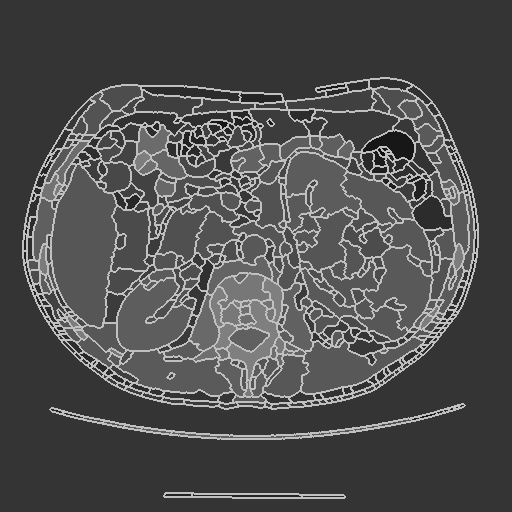
\includegraphics[width=.35\linewidth]{segmentation/segmentation-waterfall-partitionsequence-c.png}}%
	%
	\hspace{4mm}%
	%
	\subfigure[After the 2nd waterfall iteration]
	{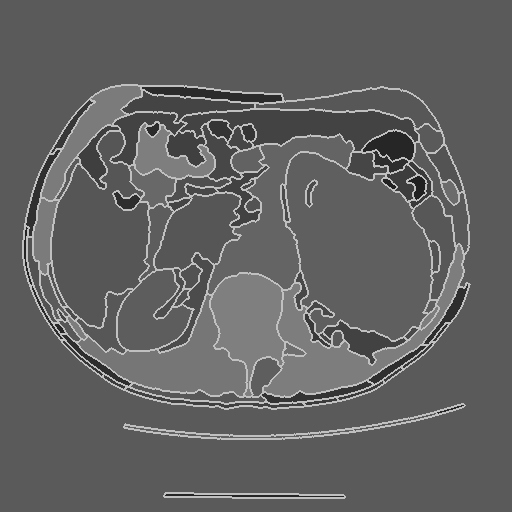
\includegraphics[width=.35\linewidth]{segmentation/segmentation-waterfall-partitionsequence-d.png}}%
	%
	\hspace{4mm}%
	%
	\subfigure[After the 3rd waterfall iteration]
	{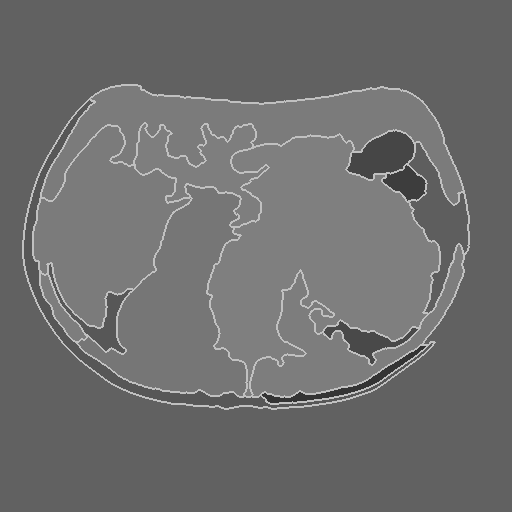
\includegraphics[width=.35\linewidth]{segmentation/segmentation-waterfall-partitionsequence-e.png}}%
	%
	\hspace{4mm}%
	%
	\subfigure[After the 4th waterfall iteration]
	{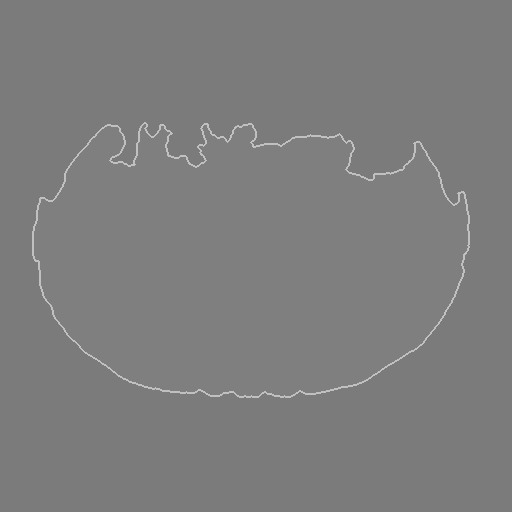
\includegraphics[width=.35\linewidth]{segmentation/segmentation-waterfall-partitionsequence-f.png}}%
\caption{An example of a waterfall partition sequence (note that the final, single-region partition is not shown). The example image was smoothed using anisotropic diffusion filtering prior to segmentation.}
\label{fig:segmentation-waterfall-partitionsequence}
\end{stusubfig}
%---

Each waterfall pass takes a partition of the landscape as input, merges some of the adjacent catchment basins together, and returns a coarser partition as its result. The input partition to the first pass is the output of an initial watershed transform on the landscape. The final partition (if we go that far) would be the whole landscape, but for most applications the regions contained in the coarsest few partitions are of little semantic interest, so the process is often terminated early.

In image terms, the waterfall helps solve the problem of oversegmentation by iteratively merging some of the regions together in a sensible way, so that regions in subsequent partitions tend both to be larger, and to correspond to semantically interesting features in the image. (This will allow us to search through all the partitions to find interesting regions, as we will see in Chapter~\ref{chap:featureid}.)

%~~~~~~~~~~~~~~~~~~~~~~~~~~~~~~~~~~~~~~~~~~~~~~~~
\subsubsection{A Waterfall Pass}
%~~~~~~~~~~~~~~~~~~~~~~~~~~~~~~~~~~~~~~~~~~~~~~~~

Conceptually, each pass of the waterfall takes its input partition (Figure~\ref{fig:segmentation-waterfall-passconcept}(a)) and transforms it into a `stepped' landscape, where there is a step corresponding to each watershed boundary, with the height of the lowest pass point along that boundary (Figure~\ref{fig:segmentation-waterfall-passconcept}(b)). It then performs a watershed transform on this stepped landscape and outputs a coarser partition of the landscape as its result (Figure~\ref{fig:segmentation-waterfall-passconcept}(c)). This process can be repeated as long as the most recent partition has more than one catchment basin (Figures~\ref{fig:segmentation-waterfall-passconcept}(d) and (e)).

%---
\begin{stusubfig}{p}
	\subfigure[The initial partition output by the watershed]
	{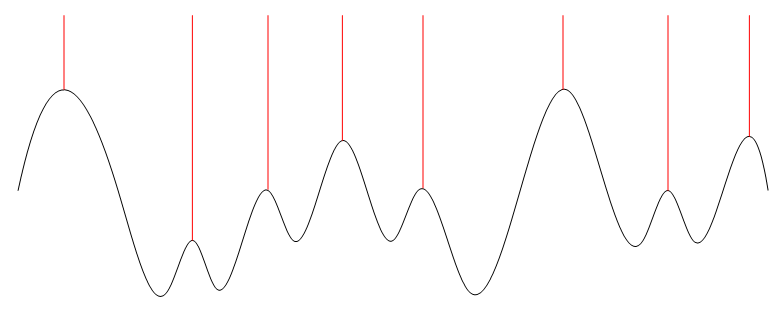
\includegraphics[width=.5\linewidth]{segmentation/segmentation-waterfall-passconcept-a.png}}%
	%
	\hspace{4mm}%
	%
	\subfigure[After transforming it into a stepped landscape]
	{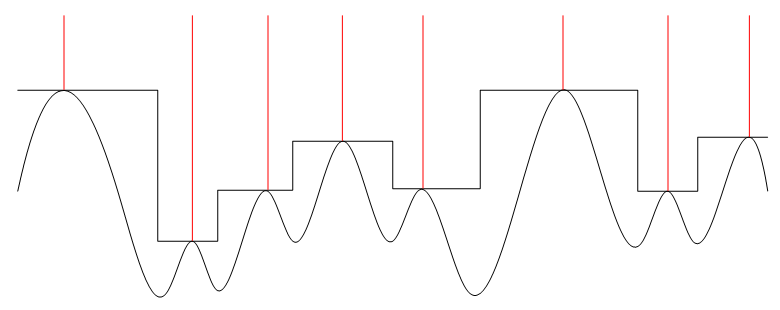
\includegraphics[width=.5\linewidth]{segmentation/segmentation-waterfall-passconcept-b.png}}%
	%
	\hspace{4mm}%
	%
	\subfigure[After performing a watershed transform on the stepped landscape]
	{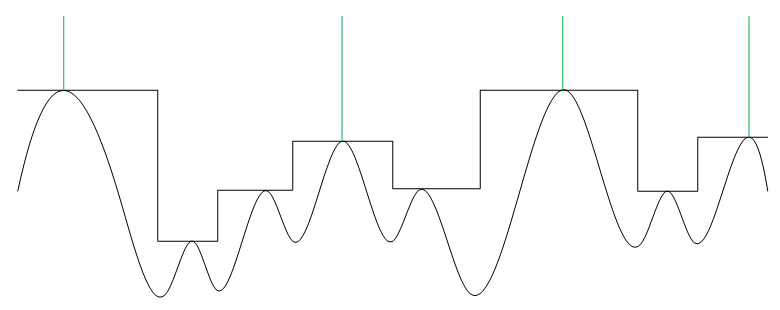
\includegraphics[width=.5\linewidth]{segmentation/segmentation-waterfall-passconcept-c.png}}%
	%
	\hspace{4mm}%
	%
	\subfigure[After the second step transformation]
	{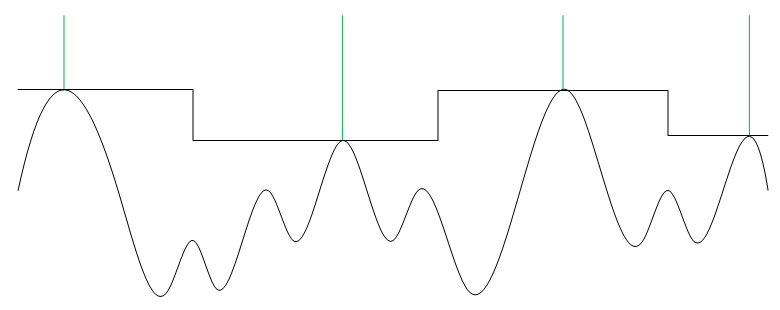
\includegraphics[width=.5\linewidth]{segmentation/segmentation-waterfall-passconcept-d.png}}%
	%
	\hspace{4mm}%
	%
	\subfigure[After performing another watershed transform]
	{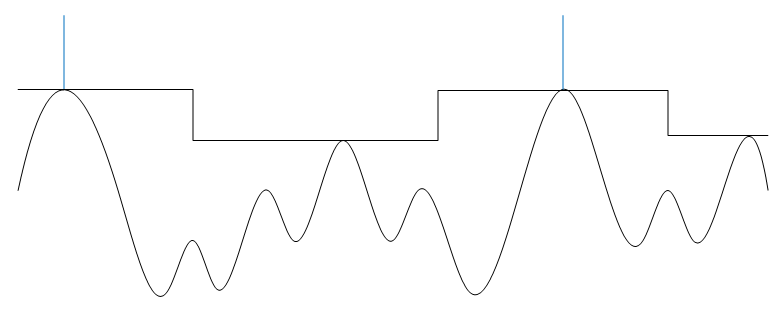
\includegraphics[width=.5\linewidth]{segmentation/segmentation-waterfall-passconcept-e.png}}%
\caption{A conceptual view of the waterfall transform}
\label{fig:segmentation-waterfall-passconcept}
\end{stusubfig}
%---

\index{waterfall transform!concept|)}

%################################################
\subsection{Practical Waterfall Algorithms}
\label{subsec:segmentation-waterfall-practicalalgorithms}
%################################################

In practice, actually transforming the landscape for each waterfall pass would be a slow process and is better avoided. More practical implementations of the waterfall are possible which work on a weighted graph whose edges correspond to watershed boundaries and whose nodes correspond to regions in the input partition (in other words, the region adjacency graph of the input partition: this is illustrated in Figure~\ref{fig:segmentation-waterfall-rag}). The weights on the graph edges, in correspondence with the conceptual description of the algorithm given above, are the heights of the lowest pass points along the corresponding watershed boundaries.

%---
\stufigex{height=8cm}{segmentation/segmentation-waterfall-rag.jpg}{An example image partition and its region adjacency graph. Note that this is an abstract diagram designed for explication purposes only: regions have been given arbitrary colours, and edges to the surrounding (beige) region and weights on all other edges have been omitted, in order to reduce unnecessary clutter in the image.}{fig:segmentation-waterfall-rag}{p}
%---

In fact, it is shown in \cite{marcotegui05} that it actually suffices to work just on a minimum spanning tree/MST (see \S\ref{sec:appendixds-rmsts}) of such a graph. Each waterfall pass then takes such an MST as its input and elides appropriate edges in it (eliding an edge means combining the nodes at either end of the edge and removing the edge itself from the MST). This has the effect of merging the partition regions joined by the edges (since the nodes which are combined actually represent regions in the partition). It is worth observing in passing (because it sheds some insight on the development of the algorithms which follow) that the goal of an MST-based waterfall algorithm is only to decide which edges in the MST need to be elided: if concerns are properly separated at a code level, the issue of how this elision process takes place can be entirely ignored for the purposes of the waterfall, and different waterfall implementations can be substituted for each other with relative impunity.

The following sections describe three different MST-based waterfall algorithms -- the first an algorithm due to Marcotegui and Beucher \cite{marcotegui05}, the second an algorithm developed by my colleague Chris Nicholls \cite{nicholls09} that is especially easy to implement, and the last my own algorithm that handles non-minimal plateaux in the MST in a more robust manner.

%~~~~~~~~~~~~~~~~~~~~~~~~~~~~~~~~~~~~~~~~~~~~~~~~
\subsubsection{Marcotegui's Algorithm}
%~~~~~~~~~~~~~~~~~~~~~~~~~~~~~~~~~~~~~~~~~~~~~~~~

\index{waterfall transform!Marcotegui's algorithm|(}

Since each waterfall pass is effectively just a graph-based waterfall transform, it can be implemented using either a flooding or a rainfalling approach. The algorithm described in \cite{marcotegui05} is an example of the former. Each pass performs a flooding-based watershed transform on MSTs, consisting of the following three steps:

\begin{enumerate}

\item \emph{Determination of Local Minima}. We define a local minimum of a weighted graph G to be a connected subgraph of G whose own edges have equal weight and whose adjacent edges in G have strictly higher weights. Figure~\ref{fig:segmentation-waterfall-marcotegui-localminima}(a) shows an example graph and its local minima. Note that the two edges with a weight of $4$ are part of the same local minimum. The first step of the algorithm consists of determining the local minima of the MST. To do this, we iterate over all the edges in the MST and flood outwards from each one to determine (a) whether it's part of a local minimum and (b) the extent of the local minimum if so.

%---
\begin{stusubfig}{p}
	\subfigure[An example graph and its local minima (drawn in red)]
	{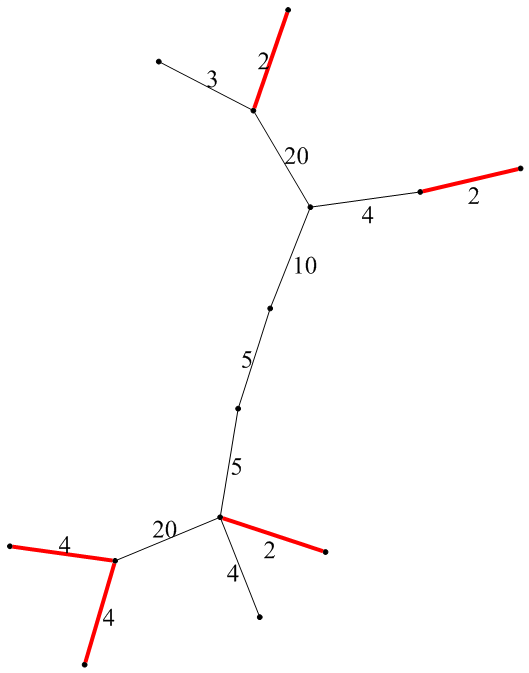
\includegraphics[width=.45\linewidth]{segmentation/segmentation-waterfall-marcotegui-graphlocalminima.png}}%
	%
	\hspace{4mm}%
	%
	\subfigure[Eliding/colouring the local minima (the edges to be elided are drawn in blue)]
	{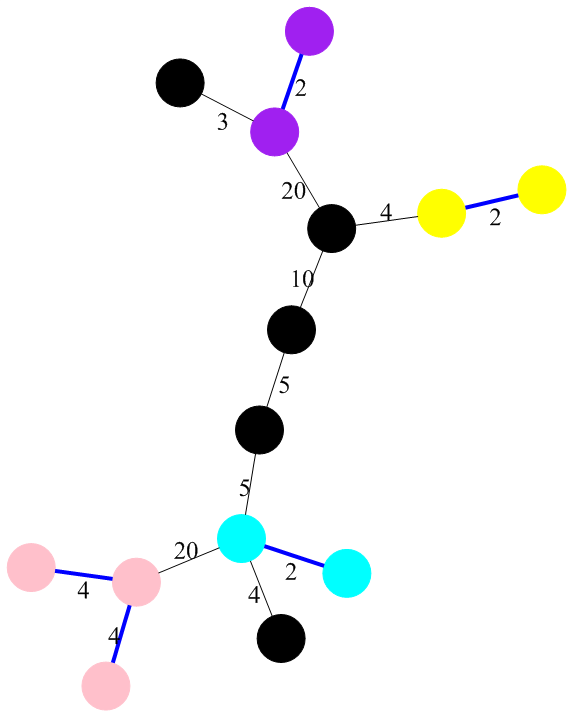
\includegraphics[width=.45\linewidth]{segmentation/segmentation-waterfall-marcotegui-localminimaelision.png}}%
\caption{Finding and eliding a graph's local minima}
\label{fig:segmentation-waterfall-marcotegui-localminima}
\end{stusubfig}
%---

%---
\begin{stusubfig}{p}
	\subfigure[The start of the propagation]
	{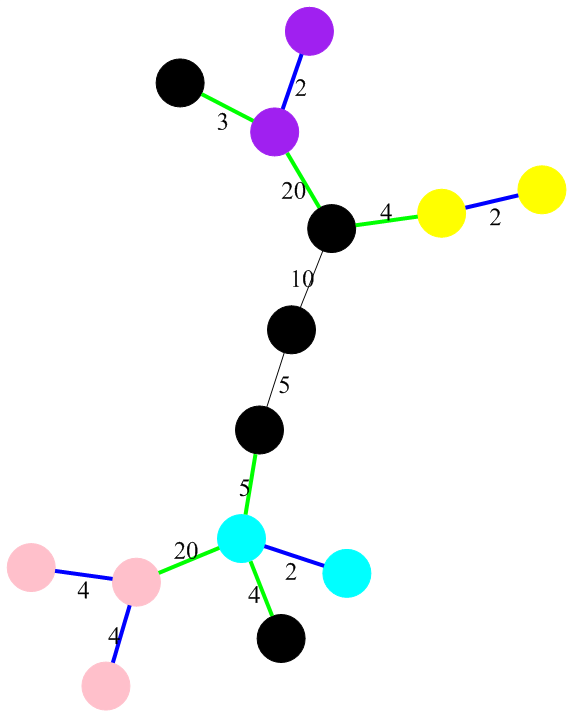
\includegraphics[width=.3\linewidth]{segmentation/segmentation-waterfall-marcotegui-propagation-a.png}}%
	%
	\hspace{4mm}%
	%
	\subfigure[The 3 edge is lowest (and elidable), so elide it]
	{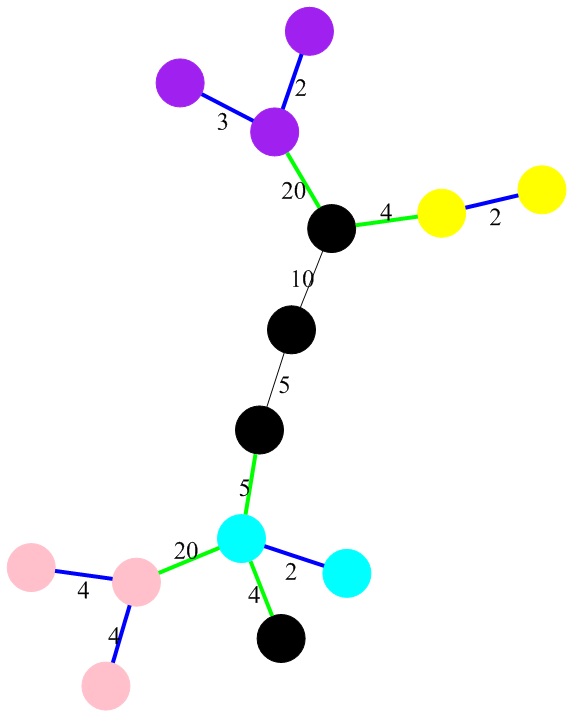
\includegraphics[width=.3\linewidth]{segmentation/segmentation-waterfall-marcotegui-propagation-b.png}}%
	%
	\hspace{4mm}%
	%
	\subfigure[A 4 edge is lowest (and elidable), so elide it]
	{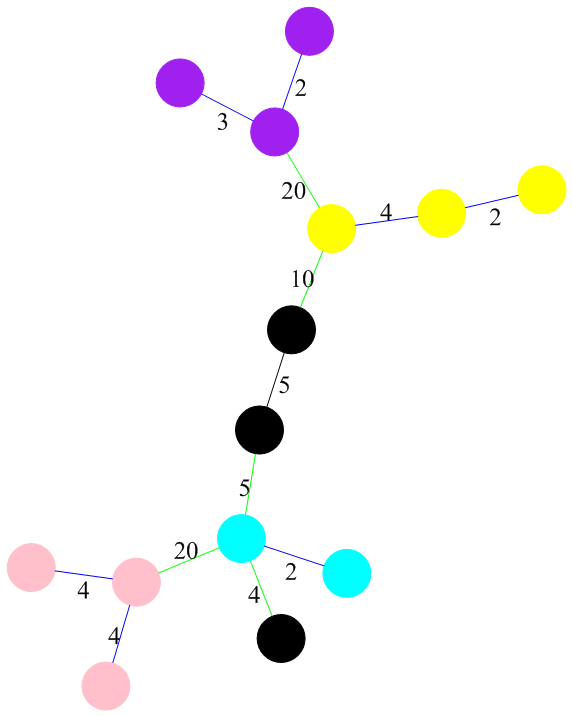
\includegraphics[width=.3\linewidth]{segmentation/segmentation-waterfall-marcotegui-propagation-c.png}}%
	%
	\hspace{4mm}%
	%
	\subfigure[The other 4 edge is lowest (and elidable), so elide it]
	{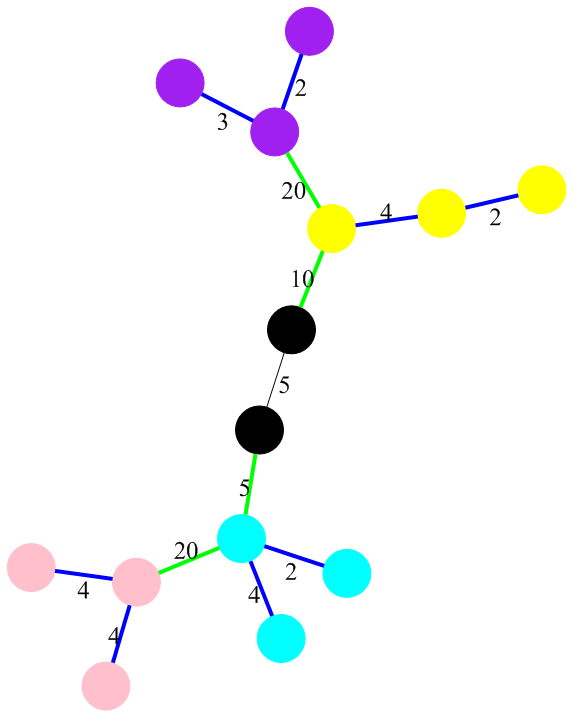
\includegraphics[width=.3\linewidth]{segmentation/segmentation-waterfall-marcotegui-propagation-d.png}}%
	%
	\hspace{4mm}%
	%
	\subfigure[The 5 edge is lowest (and elidable), so elide it]
	{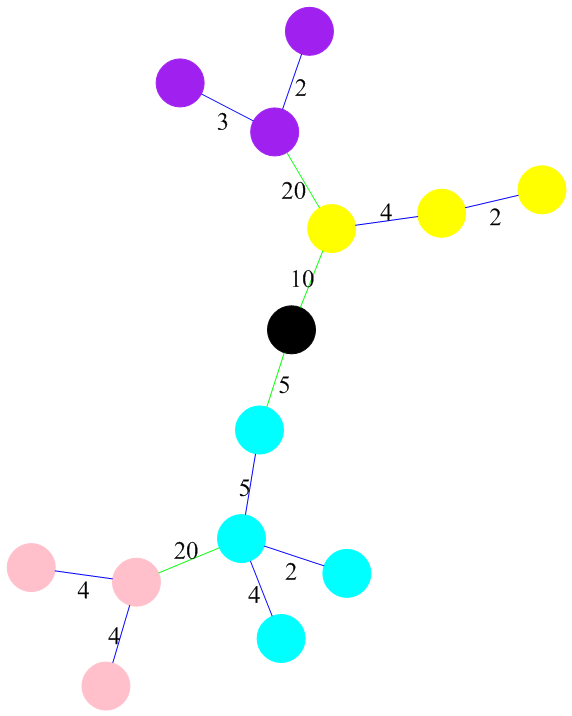
\includegraphics[width=.3\linewidth]{segmentation/segmentation-waterfall-marcotegui-propagation-e.png}}%
	%
	\hspace{4mm}%
	%
	\subfigure[The other 5 edge is lowest (and elidable), so elide it; all remaining edges will be considered in order but not elided because they are not elidable]
	{\includegraphics[width=.3\linewidth]{segmentation/segmentation-waterfall-marcotegui-propagation-f.png}}%
\caption{The propagation step of Marcotegui's waterfall algorithm, illustrated on the graph in \cite{marcotegui05}: blue edges are those that have already been elided, green edges are the ones currently under consideration, and red edges are those that will not be elided.}
\label{fig:segmentation-waterfall-marcotegui-propagation}
\end{stusubfig}
%---

\item \emph{Elision of Local Minima}. Having determined the local minima of the MST, we next elide all the edges in them: this is equivalent to merging minimal plateaux in a landscape into single points to which water can be considered to run down. In the original paper (and in the diagrams, for reasons of clarity), the nodes at the ends of an edge are assigned the same colour, rather than eliding the edge itself, but the end result is the same. See Figure~\ref{fig:segmentation-waterfall-marcotegui-localminima}(b) for an illustration.

\item \emph{Propagation}. Finally, we flood out from the nodes which now represent the local minima (so-called `marker nodes'\fxnote{[IDV] Explain connection with markers from earlier}) along the edges, in non-decreasing order of edge weight, starting from the edges directly adjacent to the marker nodes. Each edge considered will either join a marker node to another marker node, in which case it should be ignored (since eliding it would mean merging two catchment basins in the MST), or it will join a marker to a non-marker, in which case it should be elided. An illustration of the process is shown in Figure~\ref{fig:segmentation-waterfall-marcotegui-propagation}.

\end{enumerate}

\noindent A more implementation-focused description of the algorithm, including code, can be found in \cite{golodetz08}. It is important to note that the order in which edges should be processed during the propagation step is not in general well-defined (note that I wrote `non-decreasing' rather than `increasing' order of edge weight above, since multiple edges under consideration can have the same weight). The `obvious' implementation of the propagation step uses a priority queue and pops a lowest adjacent edge for consideration each time: thus the next edge to be considered ends up depending fundamentally on the way the priority queue is implemented. The consequence of this is that non-minimal plateaux in the MST are handled in a rather arbitrary way. This is not necessarily a problem in practice -- there tend to be only a small number of non-minimal plateaux in most MSTs, so it doesn't seriously affect the end result -- but it still seems slightly undesirable to have the segmentation output depend so closely on the implementation of an internal data structure which may in principle be subject to change. I will return to this issue later in this section.

\index{waterfall transform!Marcotegui's algorithm|)}

%~~~~~~~~~~~~~~~~~~~~~~~~~~~~~~~~~~~~~~~~~~~~~~~~
\subsubsection{Nicholls' Algorithm}
%~~~~~~~~~~~~~~~~~~~~~~~~~~~~~~~~~~~~~~~~~~~~~~~~

\index{waterfall transform!Nicholls' algorithm|(}

Marcotegui's waterfall method is fast and effective, but there are at least two aspects of it that can be refined. The first has just been mentioned -- the algorithm does not well-specify which edges should be elided when there are non-minimal plateaux in the MST, essentially leaving it to the implementor to make a sensible choice. I address this in my algorithm below. The second is that the algorithm as defined is a general graph algorithm, even though it is actually operating on a tree: this makes implementing the waterfall a somewhat more intricate procedure than is strictly necessary and makes the code harder to understand.

This latter problem was the motivation behind the development of a simpler, tree-based waterfall algorithm by my colleague Chris Nicholls \cite{nicholls09}. His observation was that if an edge is not elided by a waterfall pass, it is because it is a highest edge separating two adjacent catchment basins (an alternative phrasing is that it is a highest edge on the MST path between two adjacent local minima in the MST). Instead of explicitly finding the local minima in the graph and flooding out from them, therefore, it suffices to root the MST somewhere and then work recursively up from the bottom of the tree, carefully maintaining a highest edge (a `guard' edge) guarding each local minimum encountered as we go.

%---
\begin{stusubfig}{p}
	\subfigure[Before rooting the MST]
	{\includegraphics[height=6cm]{segmentation/segmentation-waterfall-nicholls-root-before.png}}%
	%
	\hspace{4mm}%
	%
	\subfigure[After rooting it]
	{\includegraphics[height=6cm]{segmentation/segmentation-waterfall-nicholls-root-after.png}}%
\caption{Nicholls' algorithm starts by picking a node at which to root the MST}% and adding a dummy root edge above the chosen root}
\label{fig:segmentation-waterfall-nicholls-root}
\end{stusubfig}
%---

%---
\begin{stusubfig}{p}
	\subfigure[The considered edge is not the unique lowest edge]
	{\includegraphics[height=5cm]{segmentation/segmentation-waterfall-nicholls-cases-a.png}}%
	%
	\hspace{4mm}%
	%
	\subfigure[The considered edge is the unique lowest edge]
	{\includegraphics[height=5cm]{segmentation/segmentation-waterfall-nicholls-cases-b.png}}%
\caption{Case analysis for the recursive step of Nicholls' algorithm: black edges are non-guards, red edges are guards, blue edges are those which have been elided and the green edge is the one under active consideration. The arrow (on the node) indicates the direction in which the algorithm presumes water to flow.}
\label{fig:segmentation-waterfall-nicholls-cases}
\end{stusubfig}
%---

%---
\begin{stusubfig}{p}
	\subfigure[Level 7]{\includegraphics[width=.17\linewidth]{segmentation/segmentation-waterfall-nicholls-example-a.png}}%
	\hspace{4mm}%
	\subfigure[Level 6]{\includegraphics[width=.17\linewidth]{segmentation/segmentation-waterfall-nicholls-example-b.png}}%
	\hspace{4mm}%
	\subfigure[Level 5]{\includegraphics[width=.17\linewidth]{segmentation/segmentation-waterfall-nicholls-example-c.png}}%
	\hspace{4mm}%
	\subfigure[Level 4]{\includegraphics[width=.17\linewidth]{segmentation/segmentation-waterfall-nicholls-example-d.png}}%
	\\
	\subfigure[Level 3]{\includegraphics[width=.17\linewidth]{segmentation/segmentation-waterfall-nicholls-example-e.png}}%
	\hspace{4mm}%
	\subfigure[Level 2]{\includegraphics[width=.17\linewidth]{segmentation/segmentation-waterfall-nicholls-example-f.png}}%
	\hspace{4mm}%
	\subfigure[Level 1]{\includegraphics[width=.17\linewidth]{segmentation/segmentation-waterfall-nicholls-example-g.png}}%
	\hspace{4mm}%
	\subfigure[Result]{\includegraphics[width=.17\linewidth]{segmentation/segmentation-waterfall-nicholls-example-h.png}}%
\caption{Nicholls' algorithm in action (considering all the edges in each level at a time for space reasons): black edges are non-guards, red edges are guards, blue edges are those which have been elided and green edges are ones under active consideration.}
\label{fig:segmentation-waterfall-nicholls-example}
\end{stusubfig}
%---

Nicholls' algorithm first roots the MST (see Figure~\ref{fig:segmentation-waterfall-nicholls-root}), adding a dummy `root edge' with a value strictly greater than the values of the edges descending from the root node (I will henceforth -- and without ambiguity -- call edges descending from a node \emph{children} of the edge ascending from that node). The value chosen is unimportant, but $\infty$ or $1$ greater than the maximum value on a child edge are sensible choices. Each pass of the algorithm is then invoked on the root edge, and proceeds recursively as follows:

%-
\begin{enumerate}

\item If the current edge is a leaf edge (i.e.~it has no child edges) then it is marked as a non-guard edge.

\item Otherwise:

%--
\begin{enumerate}

\item The algorithm is run recursively on all the child edges.

\item A child edge with minimum value is chosen (if one or more of the children with minimum value is a guard edge, one of those is chosen in preference to a non-guard). This is then referred to as the `lowest child'. The value on the current edge is compared to the value on the lowest child. If its value is less than that of the lowest child, it is marked as a non-guard edge; otherwise it is marked as a guard and the lowest child is marked as a non-guard.

\item All non-guard children are now elided.

\end{enumerate}
%--

\end{enumerate}
%-

\noindent A case analysis of what is going on should prove illuminating. There are in fact only two cases to consider: either the current edge (the parent edge) \emph{isn't} strictly the lowest leading out of a node, in which case at least part of the implied flow from the node is along the lowest child (see Figure~\ref{fig:segmentation-waterfall-nicholls-cases}(a)), or it is, in which case the implied flow from the node is entirely along the parent (see Figure~\ref{fig:segmentation-waterfall-nicholls-cases}(b)). In the first case, the algorithm arbitrarily assumes that all the implied flow is along the lowest child. In both cases, the various child edges are then elided (or not) accordingly. Figure~\ref{fig:segmentation-waterfall-nicholls-example} illustrates how the algorithm works on the same graph used to illustrate Marcotegui's algorithm above.

The assumption that all the implied flow is along the lowest child in the first case is this algorithm's way of dealing with non-minimal plateaux in the MST. As with the Marcotegui algorithm's dependence on the particular priority queue implementation used, this is a somewhat arbitrary way of handling non-minimal plateaux: in particular, the selected direction of implied flow from a particular node depends on both where the MST is rooted, and the specific method used to choose the lowest child. The algorithm also ignores the possibility that part of the implied flow is along the parent. All of this affects which specific edges are elided. As with Marcotegui's algorithm, this tends not to significantly degrade the end result, but it is still in principle desirable to devise an algorithm that does not depend on such implementation details. In the following subsection, I therefore present an alternative tree-based algorithm that handles non-minimal plateaux in the MST in a more robust manner.

\index{waterfall transform!Nicholls' algorithm|)}

%~~~~~~~~~~~~~~~~~~~~~~~~~~~~~~~~~~~~~~~~~~~~~~~~
\subsubsection{My Algorithm}
\label{subsubsec:segmentation-waterfall-myalgorithm}
%~~~~~~~~~~~~~~~~~~~~~~~~~~~~~~~~~~~~~~~~~~~~~~~~

\index{waterfall transform!my algorithm|(}

Referring back to Meijster and Roerdink's image watershed algorithm in \S\ref{subsec:segmentation-watershed-greyscale}, we observe that one robust way of dealing with the problem of non-minimal plateaux in a landscape is to first transform the image to make it lower-complete: that is, we transform it into an image where every pixel that is not within a local minimum has a lower neighbour. The method for making the image lower-complete described in \cite{meijster98} has the effect of treating pixels which are further from the border of a plateau as being in some sense `higher' than those on the boundary. The same sort of idea can be applied in the context of a waterfall pass (although it is not necessary to actually transform the MST to make it lower-complete): where there are non-minimal plateaux in the MST, we can arrange to treat the nodes further from the border of the plateaux as being `higher' than their boundary counterparts. As we will see, this enables a robust decision to be made about which edges should be elided.

The proposed algorithm is a tree-based rainfalling method, and works in three recursive passes. The first pass works up the tree from the leaf nodes, marking initial path(s) of steepest descent from each node whilst allowing for the fact that they may need to be refined later. The second pass works down the tree from the root, updating the path(s) for each node to take account of routes via parent edges and marking edges for later elision as necessary. The final pass works up the tree again to actually elide the marked edges. (This cannot be done on a down pass for technical reasons.) The MST can be rooted anywhere in order to form the input tree -- the results are the same for any choice of root. In detail, the algorithm works as follows:

%-
\begin{enumerate}

\item \emph{Up Pass}. For each node, starting from the root:

%--
\begin{enumerate}

\item Recursively process any children (the fact that the children are processed first is the reason for this being called an `up' pass).

\item If this node has a unique edge of steepest descent (i.e.~a unique lowest-valued edge leading out of it, which can be the parent edge), add an arrow on the node pointing along the edge.

\item Otherwise, consider all the lowest-valued child edges (i.e.~ignore the parent for now, even if it is also a lowest-valued edge) which satisfy the condition that there is no arrow on the node at the other end of the edge pointing along the edge towards this node. If there are no such child edges, then this node is unescapable along a child edge and should be given a distance value of $\infty$. Otherwise, each of these child edges can be assigned a distance value equal to $1$ greater than the value on the node at the other end of the edge: this value on the node will be $0$ for nodes from which there is a unique path of steepest descent, and non-zero otherwise. Pick all the child edges whose distance value is minimal and add arrows from this node pointing along them (these indicate the initial paths of steepest descent from this node). Store the minimum distance value as this node's value.

\item Now consider the parent edge: if it was a lowest-valued edge, mark it as a potential path of steepest descent to avoid the need to check again in the second pass (in Figures~\ref{fig:segmentation-waterfall-smg-pass1cases}--\ref{fig:segmentation-waterfall-smg-example}, an open-headed arrow is used to mark a parent edge for later processing).

\end{enumerate}
%--

\item \emph{Down Pass}. For each node, starting from the root:

%--
\begin{enumerate}

\item \emph{Check upwards route}.\fxnote{[IDV] Ambiguous whether upwards/downwards refer to the landscape or the tree} If a node was marked as having a potential upwards path of steepest descent, first check to make sure that there is no arrow on the parent node pointing down the edge to this node. If not, there is a possible route upwards whose distance value is $1$ greater than the value on the parent node. This is compared to any existing routes downwards via child edges. If the upwards route is strictly better, the downwards arrows are removed, the upwards route is marked and the distance value on the node is updated to reflect the better route. If the upwards route is equally good, the parent edge is marked but no other changes are made. If the upwards route is worse, it is simply ignored.

\item \emph{Check whether the parent edge (if any) should be elided}. The decision on whether or not to elide an edge is based on a classification of its two end nodes with respect to the edge itself (this is why it can only be done at this point\fxnote{[IDV] Stage?} in the algorithm). Nodes can be classified into one of five types with respect to the edge: unambiguous in (the flow from the node goes only along this edge), ambiguous in (part, but not all, of the flow from the node goes along this edge), unambiguous out (the flow from the node goes along precisely one of the other edges leading out of it), ambiguous out (the flow from the node goes along at least two of the other edges leading out of it) and no flow (there is no flow from the node at all). Based on these classifications, the parent edge is either marked for elision or not according to the case analysis shown in Figure~\ref{fig:segmentation-waterfall-smg-mergecases}. Note that there are only $13$ cases possible, rather than the expected $15$: \{ambiguous in, ambiguous in\} and \{ambiguous in, unambiguous in\} can never occur due to the way the algorithm works.

\item \emph{Recurse on any children}.

\end{enumerate}
%--

\item \emph{Up Pass}. Walk back up the tree to elide the marked edges.

\end{enumerate}
%-

%---
\begin{stusubfig}{p}
	\subfigure[UI/UI]{\includegraphics[height=5cm]{segmentation/segmentation-waterfall-smg-mergecases-uiui.png}}%
	\hspace{4mm}
	\subfigure[UI/UO]{\includegraphics[height=5cm]{segmentation/segmentation-waterfall-smg-mergecases-uiuo.png}}%
	\hspace{4mm}
	\subfigure[UO/AO]{\includegraphics[height=5cm]{segmentation/segmentation-waterfall-smg-mergecases-uiao.png}}%
	\hspace{4mm}
	\subfigure[UI/NF]{\includegraphics[height=5cm]{segmentation/segmentation-waterfall-smg-mergecases-uinf.png}}%
	\hspace{4mm}
	\subfigure[NF/NF]{\includegraphics[height=5cm]{segmentation/segmentation-waterfall-smg-mergecases-nfnf.png}}%
	\\
	\subfigure[UO/UO]{\includegraphics[height=5cm]{segmentation/segmentation-waterfall-smg-mergecases-uouo.png}}%
	\hspace{4mm}
	\subfigure[UO/AI]{\includegraphics[height=5cm]{segmentation/segmentation-waterfall-smg-mergecases-uoai.png}}%
	\hspace{4mm}
	\subfigure[UO/AO]{\includegraphics[height=5cm]{segmentation/segmentation-waterfall-smg-mergecases-uoao.png}}%
	\hspace{4mm}
	\subfigure[UO/NF]{\includegraphics[height=5cm]{segmentation/segmentation-waterfall-smg-mergecases-uonf.png}}%
	\\
	\subfigure[AO/AI]{\includegraphics[height=5cm]{segmentation/segmentation-waterfall-smg-mergecases-aoai.png}}%
	\hspace{4mm}
	\subfigure[AO/AO]{\includegraphics[height=5cm]{segmentation/segmentation-waterfall-smg-mergecases-aoao.png}}%
	\hspace{4mm}
	\subfigure[NF/AI]{\includegraphics[height=5cm]{segmentation/segmentation-waterfall-smg-mergecases-nfai.png}}%
	\hspace{4mm}
	\subfigure[NF/AO]{\includegraphics[height=5cm]{segmentation/segmentation-waterfall-smg-mergecases-nfao.png}}%
\caption{Case analysis for the edge elision step of my waterfall algorithm (a blue edge indicates that the edge would be elided; a red edge indicates that it wouldn't). The labels are AI = ambiguous in, AO = ambiguous out, NF = no flow, UI = unambiguous in and UO = unambiguous out.}
\label{fig:segmentation-waterfall-smg-mergecases}
\end{stusubfig}
%---

\noindent It is possible to perform a case analysis for the first pass and the route resolution step 2(a) as well (see Figures~\ref{fig:segmentation-waterfall-smg-pass1cases} and \ref{fig:segmentation-waterfall-smg-resolutioncases}), and this is helpful to clarify the workings of the algorithm. As illustrated in the diagram, there are six cases for the first pass: (a) the node has a unique path of steepest descent down a child edge; (b) the node has a unique path of steepest descent up the parent edge; (c) the node has more than one path of steepest descent (and the parent edge is not a possible path of steepest descent); (d) the node has more than one \emph{downwards} path of steepest descent (but the parent edge still needs to be considered); (e) there is no flow out of the node and (f) there is no downwards flow out of the node (but the parent edge still needs to be considered). For the resolution step, there are four cases: (a) the arrow from the parent node points towards us; (b) there is no flow from the parent node; (c) there is an equally good route via the parent node and (d) there is a better route via the parent node. Figure~\ref{fig:segmentation-waterfall-smg-example} illustrates how the algorithm works on the now familiar graph used to demonstrate the workings of the previous two waterfall approaches.

%---
\begin{stusubfig}{p}
	\subfigure[The node has a unique path of steepest descent down a child edge]
	{\includegraphics[width=.35\linewidth]{segmentation/segmentation-waterfall-smg-pass1cases-a.png}}%
	%
	\hspace{4mm}%
	%
	\subfigure[The node has a unique path of steepest descent up the parent edge]
	{\includegraphics[width=.35\linewidth]{segmentation/segmentation-waterfall-smg-pass1cases-b.png}}%
	%
	\hspace{4mm}%
	%
	\subfigure[The node has more than one path of steepest descent (and the parent edge is not a possible path of steepest descent)]
	{\hspace{8mm}\includegraphics[width=.35\linewidth]{segmentation/segmentation-waterfall-smg-pass1cases-c.png}\hspace{8mm}}%
	%
	\hspace{4mm}%
	%
	\subfigure[The node has more than one \emph{downwards} path of steepest descent (but the parent edge still needs to be considered)]
	{\hspace{8mm}\includegraphics[width=.35\linewidth]{segmentation/segmentation-waterfall-smg-pass1cases-d.png}\hspace{8mm}}%
	%
	\hspace{4mm}%
	%
	\subfigure[There is no flow out of the node]
	{\includegraphics[width=.35\linewidth]{segmentation/segmentation-waterfall-smg-pass1cases-e.png}}%
	%
	\hspace{4mm}%
	%
	\subfigure[There is no downwards flow out of the node (but the parent edge still needs to be considered)]
	{\hspace{8mm}\includegraphics[width=.35\linewidth]{segmentation/segmentation-waterfall-smg-pass1cases-f.png}\hspace{8mm}}%
\caption{Case analysis for the first pass of my waterfall algorithm}
\label{fig:segmentation-waterfall-smg-pass1cases}
\end{stusubfig}
%---

%---
\begin{stusubfig}{p}
	\subfigure[The arrow from the parent node points towards us]
	{\includegraphics[height=6cm]{segmentation/segmentation-waterfall-smg-resolutioncases-a.png}}%
	%
	\hspace{4mm}%
	%
	\subfigure[There is no flow from the parent node]
	{\includegraphics[height=6cm]{segmentation/segmentation-waterfall-smg-resolutioncases-b.png}}%
	%
	\hspace{4mm}%
	%
	\subfigure[There is an equally good route via the parent node]
	{\includegraphics[height=6cm]{segmentation/segmentation-waterfall-smg-resolutioncases-c.png}}%
	%
	\hspace{4mm}%
	%
	\subfigure[There is a better route via the parent node]
	{\includegraphics[height=6cm]{segmentation/segmentation-waterfall-smg-resolutioncases-d.png}}%
\caption{Case analysis for the resolution step of my waterfall algorithm (the circled node is the one currently under consideration in each case)}
\label{fig:segmentation-waterfall-smg-resolutioncases}
\end{stusubfig}
%---

%---
\begin{stusubfig}{p}
	\subfigure[The initial tree]{\includegraphics[width=.3\linewidth]{segmentation/segmentation-waterfall-smg-example-initial.png}}%
	\hspace{4mm}%
	\subfigure[After the first pass]{\includegraphics[width=.3\linewidth]{segmentation/segmentation-waterfall-smg-example-pass1.png}}%
	\hspace{4mm}%
	\subfigure[After the second pass]{\includegraphics[width=.3\linewidth]{segmentation/segmentation-waterfall-smg-example-pass2.png}}%
\caption{My waterfall algorithm running on a real example: the arrows on the nodes indicate the flow direction, blue edges are those that will be elided and red edges are those that won't be.}
\label{fig:segmentation-waterfall-smg-example}
\end{stusubfig}
%---

\index{waterfall transform!my algorithm|)}

%~~~~~~~~~~~~~~~~~~~~~~~~~~~~~~~~~~~~~~~~~~~~~~~~
\subsubsection{Comparison}
\label{subsubsec:segmentation-waterfall-comparison}
%~~~~~~~~~~~~~~~~~~~~~~~~~~~~~~~~~~~~~~~~~~~~~~~~

Each of the three waterfall algorithms just described has different properties which may make it more or less suitable to use for a given application. The key issues to consider for each algorithm are: (a) the complexity of the algorithm, (b) how easy the algorithm is to implement and (c) the nature of the resulting output, in particular regarding the robustness of the algorithm with respect to changes in implementation details. A comparison of the algorithms is presented for each of these factors.

%~~~~~~~~~~~~~~~~~~~~~~~
\paragraph{Complexity}
%~~~~~~~~~~~~~~~~~~~~~~~

The complexity of all three algorithms tends to be dominated by the construction of a minimum spanning tree for the region adjacency graph of the initial partition. As of the time of writing, the minimum spanning tree construction algorithm with the best asymptotic complexity is Chazelle's algorithm \cite{chazelle00}, which is $O(E \; \alpha(E,V))$ (where $E$ is the number of edges in the graph, $V$ is the number of vertices and $\alpha$ is the functional inverse of the Ackermann function, which grows incredibly slowly). Most practical implementations, however, are likely to use either Kruskal's algorithm ($O(E \log V)$ as most commonly implemented) or Prim's algorithm ($O(E + V \log V)$ using a Fibonacci heap).

All three waterfall algorithms converge to a partition with a single region in a very small number of iterations, so for practical purposes the number of iterations necessary can be treated as being $O(1)$.

\subparagraph{Marcotegui's Algorithm}

The complexity of the implementation of Marcotegui's algorithm suggested when it was described above is somewhat hard to characterise, due to the flooding process proposed for the implementation of step 1 of each iteration (determining the local minima of the MST). However, an iteration of Marcotegui's algorithm can be implemented in an entirely equivalent manner by running the first two passes of my waterfall algorithm on the MST to perform step 1: this classifies the edges of the MST (see Figure~\ref{fig:segmentation-waterfall-smg-mergecases}), allowing those edges which form the MST's local minima to simply be read off. In particular, the edges we are interested in are those classified as either (a) \{unambiguous in, unambiguous in\} -- a singular minimum, (b) \{unambiguous in, no flow\} -- on the boundary of a minimal plateau, or (c) \{no flow, no flow\} -- within a minimal plateau. As will be shown via the complexity analysis of my algorithm below, these can all be determined in $O(V)$ time. The edges can then be directly elided in $O(V)$ time in step 2 (note that it is unnecessary to separate them into their respective local minima, since they are all to be elided).

The analysis of the propagation process in step 3 depends on the implementation of the priority queue. Assuming the common heap-based approach \cite{clr-pq} is used, both the insertion and extraction operations on the priority queue are logarithmic in complexity. We can then observe that all the edges of the MST which did not form part of a local minimum are inserted into the priority queue once only and later extracted. Since there are (by definition) $V - 1$ edges in total in the MST, there are $O(V)$ such `non-minimal' edges, so the overall cost of the various logarithmic priority queue operations is $O(V \log V)$. The elision performed on each edge after it is extracted is $O(1)$, so the overall cost of the propagation step is $O(V \log V)$. The complexity of an iteration of Marcotegui's algorithm is thus also $O(V \log V)$, since the propagation step is the most costly part of the algorithm.

The overall complexity of Marcotegui's algorithm depends on which minimum spanning tree construction process is used. If either Kruskal's algorithm or Prim's algorithm is chosen, the complexity of that dominates the complexity of the actual iterations. In the unlikely event of Chazelle's algorithm being used, however, the complexity of the overall algorithm would be $O(E \; \alpha(E,V) + V \log V)$. This would only make sense for huge graphs, due to the constant factors involved, so we can safely discount it here.

\subparagraph{Nicholls' Algorithm}

Each iteration of Nicholls' algorithm is $O(V)$. To justify this, consider once more that there are by definition $V - 1$ edges in the MST, and that the algorithm accesses each edge a constant number of times. More specifically, each edge is processed itself, accessed again in the course of finding the lowest child of its parent, and then possibly accessed once more if it is to be elided.

The overall complexity of Nicholls' algorithm is the same as the complexity of the minimum spanning tree construction process (whichever MST algorithm is used), since the complexity of a constant number of iterations is still $O(V)$, and all the MST algorithms are $\Omega(V)$, since the original graph was connected and so $E \in \Omega(V)$.

\subparagraph{My Algorithm}

Each iteration of my algorithm is also $O(V)$. As before, we observe that there are $V - 1$ edges in the MST. Separate arguments can then be made for each of the three passes. For the first up pass, note that each edge is considered a constant number of times (once as the child edge of a node in step 1(b), once as the edge leading up from a node in 1(b), potentially once as a lowest-valued child edge in 1(c), and potentially once as a lowest-valued edge which was also the parent in 1(d)). The first up pass as a whole is thus $O(V)$. For the down pass, steps 2(a) and 2(b) involve a constant amount of work, and step 2(c) just implies that this is done for each node, so the overall amount of work is again $O(V)$. Finally, the second up pass is clearly $O(V)$, because it effectively just iterates over each edge and elides edges in $O(1)$ time where necessary. A full iteration of the algorithm is thus also $O(V)$.

The overall complexity of my algorithm is once again the same as the complexity of the minimum spanning tree construction process (whichever MST algorithm is used).

%~~~~~~~~~~~~~~~~~~~~~~~
\paragraph{Ease of Implementation}
%~~~~~~~~~~~~~~~~~~~~~~~

Of the three waterfall algorithms, Nicholls' algorithm is the easiest to implement: the iteration process itself can be implemented using a single, short, recursive function. It is particularly suitable for implementation in a functional language such as Haskell (this was a key motivation for its development), but is no harder to implement in imperative languages. My algorithm is slightly harder to implement, because it requires three separate passes over the tree for each iteration, but each pass is still simple and recursive. Marcotegui's algorithm is the hardest of the three to implement. If my algorithm is used to find the local minimum edges in preference to the flooding-based approach described earlier, however, the implementation is still relatively simple. All that is then required for each iteration is an implementation of the propagation step, which can be done straightforwardly using a priority queue, as already mentioned.

%~~~~~~~~~~~~~~~~~~~~~~~
\paragraph{Nature of Output}
%~~~~~~~~~~~~~~~~~~~~~~~

Whilst the three algorithms produce broadly similar results, the different ways in which they handle non-minimal plateaux in the MST lead to subtle differences in the output when these are present (note that the results for an MST with no non-minimal plateaux are actually identical). This variation in output is most easily understood by comparing the output of the three algorithms on an example MST with a non-minimal plateau: see Figure~\ref{fig:segmentation-waterfall-comparison}. (Note that since both Marcotegui's algorithm and Nicholls' algorithm can produce different results based on specific implementation details, only one of the possible results is shown for each.) There are a number of important things to observe:
%
\begin{enumerate}

\item Whilst Marcotegui's algorithm and Nicholls' algorithm produce results which contain the same number of regions (the number of regions produced in each case is equal to the number of local minima in the MST), my algorithm may produce a result containing more regions than the other algorithms, because it avoids making an arbitrary merging decision in ambiguous situations. This was a deliberate design choice made in the development of my algorithm: it would be easy enough to change the algorithm to instead arbitrarily pick one of the possible directions of flow from an ambiguous node in step 2(b) of my algorithm if desired.

\item The output from Nicholls' algorithm could have been generated by Marcotegui's algorithm had the order of edge extraction from the priority queue in the latter been different. The converse is also true, were the MST to be rooted at a different node. Note, however, that when faced with an ambiguous node of the type shown (the one labelled with a 1 in the result from my algorithm), Nicholls' algorithm will always choose to keep the parent edge.

\item My algorithm produces the same result regardless of where the MST is rooted. (However, in the general case, there may be multiple possible MSTs for the underlying region adjacency graph. My algorithm is \emph{not} guaranteed to produce the same result regardless of which of these is chosen, as it would be impossible for it -- or any other MST-based algorithm -- to do so. If a consistent result on the underlying graph is essential, a graph-based waterfall must be used, accepting the potential costs involved.)

\end{enumerate}

%---
\begin{stusubfig}{p}
	\subfigure[The input MST]
	{\includegraphics[width=.4\linewidth]{segmentation/segmentation-waterfall-comparison-input.png}}%
	\hspace{4mm}%
	\subfigure[A possible Marcotegui's algorithm result]
	{\includegraphics[width=.4\linewidth]{segmentation/segmentation-waterfall-comparison-marcotegui.png}}%
	\\
	\subfigure[A possible Nicholls' algorithm result]
	{\includegraphics[width=.4\linewidth]{segmentation/segmentation-waterfall-comparison-nicholls.png}}%
	\hspace{4mm}%
	\subfigure[The result of my algorithm]
	{\includegraphics[width=.4\linewidth]{segmentation/segmentation-waterfall-comparison-smg.png}}%
\caption{Comparing the outputs of the three different waterfall algorithms on a sample MST with a non-minimal plateau.}
\label{fig:segmentation-waterfall-comparison}
\end{stusubfig}
%---

%~~~~~~~~~~~~~~~~~~~~~~~
\paragraph{Summary}
%~~~~~~~~~~~~~~~~~~~~~~~

Implementing all three algorithms in \emph{millipede} revealed that for the most part they produce largely similar results for CT images, indicating that the differences in their handling of non-minimal plateaux is not a major consideration in this case in comparison to asymptotic complexity and ease of implementation. In complexity terms, all three are dominated overall by the initial construction of a minimum spanning tree, but both Nicholls' algorithm and my algorithm perform each waterfall iteration in $O(V)$ time, in comparison to $O(V \log V)$ for Marcotegui's algorithm, giving them a slight edge. In terms of ease of implementation, whilst my algorithm is relatively easy to implement, Nicholls' algorithm is clearly a particularly easy algorithm to code.

Where my algorithm could potentially have an advantage is in situations where the underlying graph might be known to have only one minimum spanning tree (perhaps because it itself is a tree) and handling of non-minimal plateaux is important. My algorithm is also useful as a way of classifying individual edges in the minimum spanning tree -- as already mentioned, this makes possible a faster (and simpler) implementation of the first step of Marcotegui's algorithm.

\index{waterfall transform|)}

\clearpage

%##################################################################################################
\section{IPF Construction}
\label{sec:segmentation-ipfconstruction}
%##################################################################################################

\index{partition forests!construction|(}

%################################################
\subsection{Overview}
%################################################

Having now seen how the watershed and waterfall transforms can be implemented, it remains to demonstrate how they can be used to construct an image partition forest as defined in the previous chapter. As mentioned in the chapter overview, I developed two separate algorithms to achieve this -- the \emph{volume-at-once} method and the \emph{subvolume} method. The goal in both cases is to construct a single IPF for the entire volume, of the type shown in Figure~\ref{fig:segmentation-ipfconstruction-goal}. The leaf layer corresponds directly to the original image, in that each node in it corresponds to a pixel in the image. The branch layers represent partitions of the image that become increasingly coarse as we ascend the forest. (Of course, the leaf layer is itself a partition of the image, if a trivial one.)

%---
\stufigex{height=20cm}{segmentation/segmentation-ipfconstruction-goal.png}{The goal of the IPF construction process: coloured edges represent tree (forest) links between layers, whilst the dotted edges in each layer represent the layer's region adjacency graph}{fig:segmentation-ipfconstruction-goal}{p}
%---

For the volume-at-once method, we observe that the image watershed algorithm described earlier can be used to produce an initial (relatively fine) partition of the image, which is then iteratively refined by the waterfall to give a sequence of ever coarser partitions. The basic idea, therefore, is that the lowest branch layer of the forest will correspond to the initial partition of the image output by the watershed, with higher branch layers being created by the waterfall; how to arrange this is described in \S\ref{subsec:segmentation-ipfconstruction-volumeatonce}.

Whilst the volume-at-once method works well for the natural approach of performing 3D segmentation on a 3D image volume, there are occasions when it is desirable to segment a 3D image volume slice by slice in a given direction, and this is the motivation for the subvolume method. For instance, if each axial slice is especially thick in comparison to the in-plane spacing between image pixels, then 3D segmentation might not always produce in-plane results that are as good as those that might be obtained by segmenting each axial slice separately. For that reason, the subvolume method divides the volume into equally-sized pieces (e.g.~2D axial slices), segments each piece separately, and then combines the results together to ultimately form a single partition forest. The details are described in \S\ref{subsec:segmentation-ipfconstruction-subvolume}. Before describing either method, however, it is first necessary to describe the way in which region properties are handled.

%~~~~~~~~~~~~~~~~~~~~~~~~~~~~~~~~~~~~~~~~~~~~~~~~
\subsubsection{Region Properties}
%~~~~~~~~~~~~~~~~~~~~~~~~~~~~~~~~~~~~~~~~~~~~~~~~

As per the description of partition forests in the previous chapter, it is possible to associate properties with forest nodes that in some way describe the regions they represent. We can use this to provide necessary information to feature identification algorithms, in particular those that will be described in the next chapter. (As a simple example, such algorithms might look for regions whose mean grey value was greater than a certain threshold, and we might arrange for a mean grey value property to be calculated for each region to support this.)

The decision about which properties to provide evidently depends on the feature identification algorithms in use. For the IPF algorithms to work, however, we have to bear in mind that it must be possible to calculate the set of properties for a particular node from the properties of its children. We will see that for certain properties (such as elongatedness), it may be necessary to augment the set of properties chosen in order to provide sufficient information in the properties of the children for this to be possible.

It is not necessary, however, for nodes in every layer to have the same set of properties: the ability to combine the properties of the children of each node to obtain the properties of the node itself is sufficient. For our application, this allows us to make a space optimization for the leaf layer, whose many nodes represent individual pixels in the image. For these nodes, there is no need to store e.g.~properties such as the area of the represented region, since it is trivially $1$ for every node in the layer. When calculating the properties of the lowest branch layer from its children in the leaf layer, it is easy enough to treat the children as having an area of $1$, without needing to explicitly store it anywhere.

%~~~~~~~~~~~~~~~~~~~~~~~
\paragraph{Chosen Property Sets}
%~~~~~~~~~~~~~~~~~~~~~~~

For the feature identification algorithms in Chapter~\ref{chap:featureid}, at least, the properties needed for a leaf node are:

%---
\begin{itemize}

\item \emph{Grey Value} ($g$). The value of the pixel in the grey value image that results from applying a CT windowing transformation to the original Hounsfield image.

\item \emph{Grey Value Gradient Magnitude} ($|\nabla g|$). The value of the pixel in the gradient magnitude of the grey value image. (This must be stored in order to calculate the edge weights between adjacent pixels on-the-fly -- storing it is less costly than storing all the actual edges.)

\item \emph{Hounsfield Value} ($h$). The original Hounsfield Unit (HU) value of the pixel.

\item \emph{Position} ($\mathbf{p}$). The position of the pixel, as a vector in either $\mathbb{R}^2$ (in 2D) or $\mathbb{R}^3$ (in 3D). (Note that careful programming can allow us to avoid storing this explicitly.)

\end{itemize}
%---

\noindent For a branch node $b$, with receptive region (i.e.~the set of leaf nodes below $b$ in the IPF) $R$, the necessary properties are:

%---
\begin{itemize}

\item \emph{Area} ($|R|$). The area of the region, in pixels.

\item \emph{Bounds} ($\mathbf{mins}$, $\mathbf{maxs}$). The minimum and maximum spatial bounds of the region, as vectors in either $\mathbb{R}^2$ (in 2D) or $\mathbb{R}^3$ (in 3D). These are defined as $\mathbf{mins}.i = \min_{\ell \in R} \mathbf{p}(\ell).i$ and $\mathbf{maxs}.i = \max_{\ell \in R} \mathbf{p}(\ell).i$ for $i \leftarrow \{x,y\}$ (in 2D) or $i \leftarrow \{x,y,z\}$ (in 3D).

\item \emph{Central Moments} ($\mu_{20}$, $\mu_{11}$, $\mu_{02}$). The $20$, $11$ and $02$ central moments of the region, all of which are scalars $\in \mathbb{R}$. The $uv$ central moment is defined as $\displaystyle \frac{1}{|R|} \sum_{\ell \in R} (x(\ell) - \bar{x}(b))^u (y(\ell) - \bar{y}(b))^v$, where $x(\ell)$ and $y(\ell)$ denote the $x$ and $y$ components of $\mathbf{p}(\ell)$, and $\bar{x}(b)$ and $\bar{y}(b)$ denote the $x$ and $y$ components of $\mathbf{c}(b)$. These statistical properties of the region are used when calculating the region's elongatedness.

\item \emph{Centroid} ($\mathbf{c}$). The centre of the region, as a vector in either $\mathbb{R}^2$ (in 2D) or $\mathbb{R}^3$ (in 3D). This is defined as $\displaystyle \frac{1}{|R|} \sum_{\ell \in R} \mathbf{p}(\ell)$.

\item \emph{Elongatedness ($e$)}. The ratio between the lengths of the major and minor axes of the minimum bounding ellipse of the region. This can be calculated using principal component analysis. In particular, if we define the covariance matrix of $R$ to be
%
\[
\left(
\begin{array}{cc}
\mu_{20} & \mu_{11} \\
\mu_{11} & \mu_{02}
\end{array}
\right),
\]
%
and calculate the eigenvalues $\lambda_1 > \lambda_2$ of this matrix, then the elongatedness of the region can be calculated as $|\sqrt{\lambda_1}| / |\sqrt{\lambda_2}|$.

\item \emph{Grey Value Max} ($M_g$). The maximum grey value of a pixel in the region. This is defined as $\displaystyle \max_{\ell \in R} g(\ell)$.

\item \emph{Grey Value Mean} ($\bar{g}$). The mean grey value of a pixel in the region, as a scalar $\in \mathbb{R}$. This is defined as $\displaystyle \frac{1}{|R|} \sum_{\ell \in R} g(\ell)$.

\item \emph{Grey Value Variance ($\upsilon_g$)}. The variance of the distribution of grey values for all pixels in the region. This is defined as $\displaystyle \frac{1}{|R|} \sum_{\ell \in R} (g(\ell) - \bar{g}(b))^2$.

\item \emph{Hounsfield Value Max} ($M_h$). The maximum HU value of a pixel in the region. This is defined as $\displaystyle \max_{\ell \in R} h(\ell)$.

\item \emph{Hounsfield Value Mean} ($\bar{h}$). The mean HU value of a pixel in the region. This is defined as $\displaystyle \frac{1}{|R|} \sum_{\ell \in R} h(\ell)$.

\item \emph{Hounsfield Value Variance ($\upsilon_h$)}. The variance of the HU distribution for all pixels in the region. This is defined as $\displaystyle \frac{1}{|R|} \sum_{\ell \in R} (h(\ell) - \bar{h}(b))^2$.

\end{itemize}
%---

\enlargethispage*{\baselineskip}

%~~~~~~~~~~~~~~~~~~~~~~~
\paragraph{Property Combination}
%~~~~~~~~~~~~~~~~~~~~~~~

\subparagraph{Branch Properties from Leaf Children}

Suppose a branch node $b$ has $k \ge 1$ (leaf) children, denoted $c_1$ to $c_k$. Then most of the properties of $b$ can be calculated directly from the definitions above (substituting the set $\{c_1,\ldots,c_k\}$ for $R$). The calculations of the variances, however, use the raw score method rather than the definition given above, as it is much more efficient. For example, for the grey value variance, this is:
%
\[
\upsilon_g(b) = \frac{\sum_{i=1}^k g(c_i)^2 - \frac{(\sum_{i=1}^k g(c_i))^2}{k}}{k}
\]

\subparagraph{Branch Properties from Branch Children}

Suppose a branch node, $b$, with pixel set $B$, has $k \ge 1$ (branch) children, $c_1$ to $c_k$, with receptive regions $C_1$ to $C_k$ respectively. We deal with the trivial properties first:

\begin{centreditemize}

\item $\displaystyle |B| = \sum_{i=1}^k |C_i|$

\item $\displaystyle \forall j \cdot \mathbf{mins}(b).j = \min_{i=1}^k \mathbf{mins}(c_i).j$

\item $\displaystyle \forall j \cdot \mathbf{maxs}(b).j = \max_{i=1}^k \mathbf{maxs}(c_i).j$

\item $\displaystyle \mathbf{c}(b) = \frac{1}{|B|} \sum_{i=1}^k |C_i| \mathbf{c}(c_i)$

\item $\displaystyle M_g(b) = \max_{i=1}^k M_g(c_i)$

\item $\displaystyle \bar{g}(b) = \frac{1}{|B|} \sum_{i=1}^k |C_i| \bar{g}(c_i)$

\item $\displaystyle M_h(b) = \max_{i=1}^k M_h(c_i)$

\item $\displaystyle \bar{h}(b) = \frac{1}{|B|} \sum_{i=1}^k |C_i| \bar{h}(c_i)$

\end{centreditemize}

\noindent Combining the grey value variances of the children to find the parent variance is slightly more involved. We observe that:
%
\begin{eqnarray*}
&   & |B|\upsilon_g(b) \\
& = & \sum_{\ell \in B} (g(\ell) - \bar{g}(b))^2 \\
& = & \sum_{i=1}^k \sum_{\ell \in C_i} (g(\ell) - \bar{g}(b))^2
\end{eqnarray*}
%
\noindent Furthermore:
%
\[
\sum_{i=1}^k |C_i|\upsilon_g(c_i) = \sum_{i=1}^k \sum_{\ell \in C_i} (g(\ell) - \bar{g}(c_i))^2
\]
%
\noindent Thus:
%
\begin{eqnarray*}
&   & |B|\upsilon_g(b) - \sum_{i=1}^k |C_i|\upsilon_g(c_i) \\
%
& = & \sum_{i=1}^k \sum_{\ell \in C_i} \left\{ (g(\ell) - \bar{g}(b))^2 - (g(\ell) - \bar{g}(c_i))^2 \right\} \\
%
& = & \sum_{i=1}^k \sum_{\ell \in C_i} (2g(\ell) - \bar{g}(b) - \bar{g}(c_i))(\bar{g}(c_i) - \bar{g}(b)) \\
%
& = & \sum_{i=1}^k (\bar{g}(c_i) - \bar{g}(b)) \left\{ 2 \sum_{\ell \in C_i} g(\ell) - \sum_{\ell \in C_i} (\bar{g}(b) + \bar{g}(c_i)) \right\} \\
%
& = & \sum_{i=1}^k (\bar{g}(c_i) - \bar{g}(b)) \left\{ 2|C_i|\bar{g}(c_i) - |C_i|(\bar{g}(b) + \bar{g}(c_i)) \right\} \\
%
& = & \sum_{i=1}^k |C_i|(\bar{g}(c_i) - \bar{g}(b))^2
\end{eqnarray*}
%
\noindent This in turn gives us the required formula, namely:
%
\[
\upsilon_g(b) = \frac{1}{|B|} \sum_{i=1}^k |C_i| (\upsilon_g(c_i) + (\bar{g}(c_i) - \bar{g}(b))^2)
\]
%
\noindent The formula for the Hounsfield value variance is entirely analogous. A similar approach also works for the central moments, which can be combined using the formula:
%
\[
\mu_{uv}(b) = \frac{1}{|B|} \sum_{i=1}^k |C_i| (\mu_{uv}(c_i) + (\bar{x}(c_i) - \bar{x}(b))^u (\bar{y}(c_i) - \bar{y}(b))^v)
\]
%
\noindent The elongatedness of $b$ is calculated not by combining the elongatedness properties of the child nodes, but by direct calculation from the calculated central moments for $b$ (via principal component analysis, as described earlier).

%################################################
\subsection{The Volume-at-once Method}
\label{subsec:segmentation-ipfconstruction-volumeatonce}
%################################################

\index{partition forests!construction!volume-at-once method|(}

Recall from the section overview that the goal of both the IPF construction methods presented in this thesis is to build the type of IPF shown in Figure~\ref{fig:segmentation-ipfconstruction-goal}. There are three key issues to be tackled in each case:
%
\begin{enumerate}
\item How to construct the leaf layer from the input Hounsfield image.
\item How to construct the lowest branch layer (intuitively corresponding to the watershed result).
\item How to construct the higher branch layers (intuitively corresponding to the sequence of waterfall results).
\end{enumerate}
%
The volume-at-once method deals with each of these issues as follows. The leaf layer is constructed directly from the Hounsfield image, with a one-to-one correspondence between leaf layer nodes and image voxels. The lowest branch layer is constructed directly from the result of running a watershed algorithm on the whole of the (pre-processed) source image. Each higher branch layer is constructed by cloning the current top-most layer of the forest and using a waterfall iteration to merge some of the regions in the clone together in order to form a coarser partition of the original image. The details of each of these processes are now examined in more detail.

%~~~~~~~~~~~~~~~~~~~~~~~~~~~~~~~~~~~~~~~~~~~~~~~~
\subsubsection{Constructing the Leaf Layer}
%~~~~~~~~~~~~~~~~~~~~~~~~~~~~~~~~~~~~~~~~~~~~~~~~

In essence, constructing a leaf layer from a Hounsfield image is a fairly simple process. The Hounsfield image is first windowed (as discussed in \S\ref{subsubsec:segmentation-watershed-ct-windowing}) to produce the `grey value' image. This is then smoothed using anisotropic diffusion filtering to produce the `grey value gradient magnitude' image. Finally, these three images are passed as input to the leaf layer construction process, which creates a leaf node for each image voxel location and extracts the leaf node properties for that voxel -- i.e.~the grey value, grey value gradient magnitude and Hounsfield value, as per the previous section -- from their respective images. (Note that voxel position is not stored as a leaf node property, as it can be inferred from the index of a leaf node and the dimensions of the input images.)

It remains to specify the region adjacency graph (RAG) for the leaf layer. As Figure~\ref{fig:segmentation-ipfconstruction-goal} indicates, this simply connects every voxel to its neighbours (recalling that neighbourhood depends on what notion of connectivity we chose: see Figure~\ref{fig:segmentation-watershed-connectivity}). This regularity makes it possible for sensible implementations to avoid storing the (many) edges of the leaf layer graph explicitly, a desirable aim given the generally large sizes of the images involved. Instead, edges and their weights are calculated on demand. An edge between adjacent voxels is weighted with the maximum of the two gradient magnitude values stored at the voxels (note that this is why gradient magnitude values are a leaf node property), as this provides an appropriate measure of the height of the boundary between them in the grey value gradient magnitude image. When a request is made for the adjacent edges or adjacent nodes of a particular voxel, the relevant set is constructed on-the-fly.

%~~~~~~~~~~~~~~~~~~~~~~~~~~~~~~~~~~~~~~~~~~~~~~~~
\subsubsection{Constructing the Lowest Branch Layer}
%~~~~~~~~~~~~~~~~~~~~~~~~~~~~~~~~~~~~~~~~~~~~~~~~

At a high level, the lowest branch layer of the forest is constructed by running a watershed algorithm (in our case, Meijster and Roerdink's watershed algorithm, as described in \S\ref{subsubsec:segmentation-watershed-meijster}) on the grey value gradient magnitude image and constructing a node corresponding to each catchment basin in the watershed result. Forest links are then added between each catchment basin node in the lowest branch layer and the leaf layer nodes corresponding to the voxels it contains. Finally, the edges between the voxels in the leaf layer are propagated upwards (in a manner that will be described shortly) to form the RAG for the lowest branch layer.

In implementation terms, the process works as follows. We first perform a raster scan over the label image produced by the watershed to group the voxels into their respective catchment basins. The voxel groups are then passed to the lowest branch layer builder, which creates a node for each group (i.e.~for each catchment basin), adds forest links between the node and its children in the leaf layer, and calculates the node's properties from those of its children, as described earlier under \emph{Branch Properties from Leaf Children}. Finally, we iterate over all the edges in the leaf layer. We compare the weight on each child edge $(c_i,c_j)$ against the weight on the current edge (if any) between $\mbox{parent}(c_i)$ and $\mbox{parent}(c_j)$ in the lowest branch layer. If it is lower than the existing weight (or there is currently no such edge), we set the weight on the parent edge to be the weight on the child edge. This has the effect of adding all the relevant edges to the lowest branch layer RAG, each weighted with the lowest pass point on the boundary between the adjacent regions joined. Figure~\ref{fig:segmentation-ipfconstruction-lowestbranchlayer} illustrates the desired results on an example $3 \times 3$ image.

%---
\begin{stusubfig}{p}
	\subfigure[The leaf layer and its 4-connected RAG (the letters on the pixels are leaf node references; the numbers are the pixel values)]
	{\includegraphics[width=.45\linewidth]{segmentation/segmentation-ipfconstruction-lowestbranchlayer-a.png}}%
	%
	\hspace{12mm}%
	%
	\subfigure[The watershed labelling (shown as a colouring on the nodes)]
	{\includegraphics[width=.45\linewidth]{segmentation/segmentation-ipfconstruction-lowestbranchlayer-b.png}}%
	%
	\\ \vspace{4mm}
	%
	\subfigure[The lowest branch layer and its RAG (the edges are shown as being between the original pixels they connect for illustration purposes, but are really a--b, a--e and b--e in the lowest branch layer)]
	{\includegraphics[width=.45\linewidth]{segmentation/segmentation-ipfconstruction-lowestbranchlayer-c.png}}%
	%
	\hspace{12mm}%
	%
	\subfigure[The forest structure of the lowest two layers]
	{\includegraphics[width=.45\linewidth]{segmentation/segmentation-ipfconstruction-lowestbranchlayer-d.png}}%
\caption{The lowest two layers of the partition forest}
\label{fig:segmentation-ipfconstruction-lowestbranchlayer}
\end{stusubfig}
%---

It will be seen in the next section that there is actually an alternative to constructing the lowest branch layer explicitly in the manner described above. A general scheme for adding a coarser partition to the top of the forest is to clone the current top-most layer of the IPF, and then merge some of the nodes in the new top-most layer in a manner decided by a segmentation algorithm (e.g.~the watershed). In theory, therefore, we could have cloned the leaf layer to form the lowest branch layer, then merged some of its nodes together based on the watershed labelling. This would have allowed us to avoid explicitly calculating the required RAG for the lowest branch layer. Unfortunately, it may not always be practical in environments with limited storage.\footnote{This is not to say that the approach is never practical: in environments with sufficient memory, it may actually be preferable, because it is somewhat simpler than the alternative.} The leaf layer's RAG, whilst extremely large, can be stored implicitly because it is entirely regular. The RAG for the lowest branch layer, however, is not regular. In its final form, it is also not especially large (thus posing no inherent storage problem), but the scheme described above works by gradually transforming the large leaf layer RAG into the smaller RAG of the lowest branch layer, via a process of merging some of its nodes together. The non-regular intermediate graph (which is initially almost as large as the leaf layer graph) must be stored explicitly, and it is this which potentially causes a problem. An alternative approach of storing just the differences between the leaf layer graph and the intermediate graph just alters the problem, without in any way solving it. For that reason, the explicit way of constructing the lowest branch layer is a preferable approach, despite involving slightly more work.

%~~~~~~~~~~~~~~~~~~~~~~~~~~~~~~~~~~~~~~~~~~~~~~~~
\subsubsection{Constructing the Higher Branch Layers}
%~~~~~~~~~~~~~~~~~~~~~~~~~~~~~~~~~~~~~~~~~~~~~~~~

%---
\begin{stulisting}[p]
\caption{The Volume-at-once Waterfall Listener}
\label{code:segmentation-ipfconstruction-volumeatonce-waterfalllistener}
\begin{lstlisting}[style=Default,language=C++]
template <typename Forest>
struct VolumeAtOnceWaterfallPassListener
:	public WaterfallPass<typename Forest::EdgeWeight>::Listener
{
	//...

	void merge_nodes(int u, int v)
	{
		// Merge the corresponding nodes in the top-most layer of the forest.
		std::set<PFNodeID> mergees;
		mergees.insert(PFNodeID(m_forest->highest_layer(), u));
		mergees.insert(PFNodeID(m_forest->highest_layer(), v));
		m_forest->merge_sibling_nodes(mergees, Forest::DONT_CHECK_PRECONDITIONS);
	}
};
\end{lstlisting}
\end{stulisting}
%---

%---
\begin{stusubfig}{p}
	\subfigure[A forest after constructing the lowest two layers]
	{\hspace{4mm}\includegraphics[width=.45\linewidth]{segmentation/segmentation-ipfconstruction-higherlayers-a.png}\hspace{4mm}}%
	%
	\\
	%
	\subfigure[After cloning the top-most layer]
	{\includegraphics[width=.45\linewidth]{segmentation/segmentation-ipfconstruction-higherlayers-b.png}}%
	%
	\hspace{4mm}%
	%
	\subfigure[After the first waterfall iteration]
	{\includegraphics[width=.45\linewidth]{segmentation/segmentation-ipfconstruction-higherlayers-c.png}}%
	%
	\\
	%
	\subfigure[After cloning the top-most layer]
	{\includegraphics[width=.45\linewidth]{segmentation/segmentation-ipfconstruction-higherlayers-d.png}}%
	%
	\hspace{4mm}%
	%
	\subfigure[After the second waterfall iteration]
	{\includegraphics[width=.45\linewidth]{segmentation/segmentation-ipfconstruction-higherlayers-e.png}}%
\caption{Constructing the higher branch layers of a partition forest using the volume-at-once method}
\label{fig:segmentation-ipfconstruction-higherlayers}
\end{stusubfig}
%---

The higher branch layers of the forest are constructed using the waterfall transform. The waterfall algorithms presented in \S\ref{sec:segmentation-waterfall}, however, operate not on a region adjacency graph, but on a minimum spanning tree; before they can be used, therefore, it is necessary to construct an MST of the lowest branch layer's RAG. This can be done in a variety of standard ways (see Listing~\ref{code:appendixds-rootedmst-construction} for the implementation used here).

Having constructed the MST, we then iteratively clone the top-most layer of the forest and run a waterfall iteration (of whichever algorithm we decide to use) on the MST. When the waterfall iteration calls for an edge to be elided, we arrange for this to not only elide the edge in the MST, but merge the relevant regions in the top-most layer of the forest as well. To do this, we modify the waterfall algorithms to support external listeners, which are informed when an edge in the MST is merged. We then add a listener that merges the corresponding regions in the top-most forest layer (see Listing~\ref{code:segmentation-ipfconstruction-volumeatonce-waterfalllistener}). The MST itself is maintained from one iteration of the waterfall to the next: at the beginning of each waterfall iteration it is the MST for the current top-most layer of the forest. This allows us to avoid rebuilding the MST for each new iteration. Figure~\ref{fig:segmentation-ipfconstruction-higherlayers} illustrates how the construction of the higher branch layers of a forest might proceed. The process continues either for a fixed number of iterations, or until the top-most layer of the forest contains only a single region. The result is the finished partition forest for the image, which is suitable for further processing.

\index{partition forests!construction!volume-at-once method|)}

%################################################
\subsection{The Subvolume Method}
\label{subsec:segmentation-ipfconstruction-subvolume}
%################################################

\index{partition forests!construction!subvolume method|(}

The volume-at-once method described in the previous section only allows a 3D image volume to be segmented using 3D segmentation. This is the natural approach, but there are times when it can be desirable to segment individual slices in 2D and then combine the results to form a single partition forest for further editing: this is the purpose of the subvolume method.

%~~~~~~~~~~~~~~~~~~~~~~~~~~~~~~~~~~~~~~~~~~~~~~~~
\subsubsection{Constructing the Lowest Layers}
%~~~~~~~~~~~~~~~~~~~~~~~~~~~~~~~~~~~~~~~~~~~~~~~~

The subvolume method starts by generating the leaf layer and lowest branch layer for the overall volume. An example of the way this works for a volume containing three slices is shown in Figure~\ref{fig:segmentation-ipfconstruction-subvolumemethod-lowestlayers}. The first step is to split the 3D image volume into its constituent subvolumes (the slices, in the example) -- these must all be the same size. For each subvolume, we then construct a separate leaf layer and lowest branch layer, using the approaches described for the volume-at-once method -- in particular, a watershed algorithm is applied to segment each subvolume separately. Finally, the leaf layers for the various subvolumes are combined into a leaf layer for the overall volume, and the lowest branch layers for the subvolumes are combined to form the volume's lowest branch layer.

%---
\stufigex{height=19cm}{segmentation/segmentation-ipfconstruction-subvolumemethod-lowestlayers.png}{Constructing the lowest two layers using the subvolume method -- the image volume is divided into equally-sized pieces, each of which has a leaf layer ($\mathit{LL}$) and lowest branch layer ($\mathit{LBL}$) constructed for it as per the volume-at-once method. The corresponding layers are then combined together again to produce the leaf layer and lowest branch layer for the volume as a whole. This example works on a volume with three slices, but the approach generalises in the natural way.}{fig:segmentation-ipfconstruction-subvolumemethod-lowestlayers}{p}
%---

%~~~~~~~~~~~~~~~~~~~~~~~~~~~~~~~~~~~~~~~~~~~~~~~~
\subsubsection{Constructing the Higher Layers}
%~~~~~~~~~~~~~~~~~~~~~~~~~~~~~~~~~~~~~~~~~~~~~~~~

%---
\begin{stulisting}[p]
\caption{The Subvolume Waterfall Listener}
\label{code:segmentation-ipfconstruction-subvolume-waterfalllistener}
\begin{lstlisting}[style=Default,language=C++]
template <typename Forest>
struct SubvolumeWaterfallPassListener
:	public WaterfallPass<typename Forest::EdgeWeight>::Listener
{
	//...

	SubvolumeWaterfallPassListener(const Forest_Ptr& forest,
								   const SubvolumeToVolumeIndexMapper& indexMapper)
	:	m_forest(forest), m_indexMapper(indexMapper)
	{}

	void merge_nodes(int u, int v)
	{
		// Merge the corresponding nodes in the top-most layer of the forest.
		std::set<PFNodeID> mergees;
		mergees.insert(PFNodeID(m_forest->highest_layer(), m_indexMapper(u)));
		mergees.insert(PFNodeID(m_forest->highest_layer(), m_indexMapper(v)));
		m_forest->merge_sibling_nodes(mergees, Forest::DONT_CHECK_PRECONDITIONS);
	}
};

int SubvolumeToVolumeIndexMapper::operator()(int nodeIndex) const
{
	// Step 1:	Calculate the position relative to the start of the subvolume.
	itk::Index<3> subvolPos = {{
		GridUtil::x_of(nodeIndex, m_subvolumeSize[0]),
		GridUtil::y_of(nodeIndex, m_subvolumeSize[0], m_subvolumeSize[1]),
		GridUtil::z_of(nodeIndex, m_subvolumeSize[0] * m_subvolumeSize[1])
	}};

	// Step 2:	Offset by the position of the start of the subvolume.
	itk::Index<3> volPos = subvolPos + m_subvolumeStart;

	// Step 3:	Convert to a volume index.
	return (volPos[2] * m_volumeSize[1] + volPos[1]) * m_volumeSize[0] + volPos[0];
}
\end{lstlisting}
\end{stulisting}
%---

%---
\stufigex{height=6cm}{segmentation/segmentation-ipfconstruction-subvolumemethod-anysize.png}{One of the waterfall partitions resulting from segmenting a $512 \times 512 \times 1$ image in $64 \times 64 \times 1$ chunks}{fig:segmentation-ipfconstruction-subvolumemethod-anysize}{p}
%---

Constructing the higher layers is somewhat more intricate. We want to be able to run a waterfall algorithm on each of the subvolumes separately (thus separately segmenting each subvolume), whilst still only constructing a single partition forest for the entire volume. To do this, we can start by building a minimum spanning tree for each subvolume's lowest branch layer and running a waterfall algorithm on it, just as we might in the volume-at-once method. However, because this time we are working with subvolumes, the waterfall in this case will call for nodes to be merged based on their indices in the individual subvolume's forest, not in the forest for the volume as a whole. Clearly, this presents us with a problem.

The trick here is in how we implement the waterfall listener (see Listing~\ref{code:segmentation-ipfconstruction-subvolume-waterfalllistener}). Unlike the volume-at-once waterfall listener (see Listing~\ref{code:segmentation-ipfconstruction-volumeatonce-waterfalllistener}), this one maps the indices of the nodes to be merged in a subvolume's forest to their counterparts in the overall volume's forest before performing the merge on the the overall forest. The details of this process are not especially important here -- all that matters is that this allows us to run separate waterfall processes on each of the subvolumes whilst constructing a single partition forest for the volume as a whole.

As a side note, it is worth observing that the subvolume method described here is not restricted to segmenting image volumes slice by slice -- it can be used to segment them using subvolumes of any size, provided that the subvolume dimensions divide evenly into those of the overall volume. For instance, Figure~\ref{fig:segmentation-ipfconstruction-subvolumemethod-anysize} shows the results of segmenting a $512 \times 512 \times 1$ image in $64 \times 64 \times 1$ chunks. Whilst primarily an implementation quirk at present, this does have potential uses. For instance, there is in principle no reason why the approach could not be extended to arbitrary subvolume sizes, at the expense of a far more complicated implementation, which might actually be useful if the user wanted to segment separate sections of the body using different segmentation parameters.

\index{partition forests!construction!subvolume method|)}
\index{partition forests!construction|)}

\newpage

%##################################################################################################
\section{Chapter Summary}
%##################################################################################################

In this chapter, we saw how to generate IPFs from medical images using the morphological watershed and waterfall transforms. The next chapter will show how the generated IPFs can be used when automatically identifying salient features in the original images.
